\documentclass[abstract=on,10pt,a4paper,bibliography=totocnumbered]{scrartcl}
\usepackage[utf8]{inputenc}
\usepackage[english]{babel}
\usepackage{amsmath}
\usepackage{colortbl}
\usepackage{amsfonts}
\usepackage{amssymb}
\usepackage{graphicx}
\usepackage{enumerate}
\usepackage{epstopdf}
\usepackage[onehalfspacing]{setspace}
\usepackage[paper=a4paper,left=30mm,right=30mm,top=20mm,bottom=25mm]{geometry}
\usepackage[round]{natbib}
\usepackage[hidelinks]{hyperref}
\usepackage[nameinlink]{cleveref}
\usepackage{multirow}
\usepackage{booktabs}
\usepackage[labelfont=bf]{caption}
\usepackage{footnote}
\usepackage{tabularx}
\usepackage{gensymb}
\usepackage{todonotes}
\usepackage{tikz}
\usepackage{subcaption}
\usepackage{varwidth}
% \usepackage[nomarkers,figuresonly]{endfloat}
\usepackage{csvsimple}
\usepackage{arydshln}
\usepackage{titlesec}

% Define a new command to create a number inside a circle (for plots)
\newcommand*\circled[1]{\tikz[baseline=(char.base)]{
            \node[shape=circle,draw,inner sep=1pt] (char) {#1};}}

% Creating some TikZ styles
\tikzset{
  nonterminal/.style = {rectangle
    , minimum size = 6mm
    , very thick
    , draw = black!
  }
}

% Increase the space between two rows in tables
\renewcommand{\arraystretch}{1.2}

% Changing the style of captions in figures etc.
\captionsetup{labelfont=bf, format=plain, font=small}

% Adjust the distance between title and paragraph
\RedeclareSectionCommand[
  beforeskip=-.5\baselineskip,
  afterskip=.5\baselineskip]{subsection}
\RedeclareSectionCommand[
  beforeskip=-.25\baselineskip,
  afterskip=.25\baselineskip]{subsubsection}

\doublespacing
\begin{document}
\pagenumbering{gobble}
\bibliographystyle{apalike}

\begin{titlepage}

% Define a new command to produce a horizontal line
\newcommand{\HRule}{\rule{\linewidth}{0.5mm}}

% Center everything on the page
\center

%------------------------------------------------------------------------------
%	HEADING SECTIONS
%------------------------------------------------------------------------------

% Name of your university/college
\textsc{\LARGE  }\\[1.5cm]

% Major heading
\textsc{\Large Department of Evolutionary Biology and Environmental
Studies}\\[0.5cm]

% Minor heading
\textsc{\large Master's Thesis}\\[0.5cm]

%------------------------------------------------------------------------------
%	TITLE SECTION
%------------------------------------------------------------------------------
\doublespacing
\HRule \\[0.4cm]

% Title of the document
{\textsc{ \LARGE On the Move: Dispersal Corridors of African Wild Dogs
(\textit{Lycaon pictus}) in the Kavango-Zambezi Transfrontier Conservation
Area}}\\[0.4cm]

\HRule \\[1.5cm]
\singlespacing

%------------------------------------------------------------------------------
%	AUTHOR SECTION
%------------------------------------------------------------------------------

\begin{minipage}{0.4\textwidth}
\begin{flushleft} \large

% Main author
\emph{Author:}\\
David D. Hofmann\\
david.hofmann2@uzh.ch\\
12-728-846

\end{flushleft}
\end{minipage}
~
\begin{minipage}{0.4\textwidth}
\begin{flushright} \large

% Supervisors
\emph{Supervisors:} \\
Dominik Behr\\
Ph.D. Gabriele Cozzi\\
Prof. Arpat Ozgul

\end{flushright}
\end{minipage}\\[2cm]

%------------------------------------------------------------------------------
%	DATE SECTION
%------------------------------------------------------------------------------

% Today's date
{\large \today}\\[5cm]

%------------------------------------------------------------------------------
%	LOGO SECTION
%------------------------------------------------------------------------------

% Logo of the university

\includegraphics{UZHVector.eps}\\[1cm]

%------------------------------------------------------------------------------

% Fill the rest of the page with whitespace
\vfill

\end{titlepage}

\begin{abstract}
The African wild dog \textit{(Lycaon pictus)} is an endangered species that
currently only survives in a few scattered subpopulations in Sub-Saharan Africa.
Long-term viability of the species thus requires to identify and preserve key
dispersal corridors that connect such subpopulations. We collected GPS data of
16 dispersing coalitions originating from a free-ranging population in northern
Botswana and used integrated step selection analysis to create a permeability
surface spanning over the entire Kavango-Zambezi Transfrontier Conservation Area
(KAZA-TFCA), the largest transboundary conservation area on earth. Based on our
permeability surface, we calculated least-cost paths and least-cost corridors
between selected locations within the KAZA-TFCA. Our results show that dispersal
corridors typically run through open shrubs/grassland and in the vicinity of
water. Corridors rarely cross water bodies, areas with high human presence, or
areas densely vegetated by trees. Several dispersal corridors meet in the
Okavango-Linyanty ecosystem, which highlights the importance of northern
Botswana for the conservation of this charismatic species.
\end{abstract}
\newpage

\onehalfspacing
\tableofcontents
\doublespacing
\newpage

\pagenumbering{arabic}

\section{Introduction}
% Importance of Connectivity
Successful conservation of fragmented and isolated subpopulations requires to
maintain and enhance connectivity between habitats occupied by these
subpopulations \citep{Hanski.1998}. In this context, connectivity describes the
degree to which the landscape matrix facilitates or impedes movements of
individuals of the focal species between habitat patches \citep{Taylor.1993,
Clobert.2012}. Thus, sufficient connectivity facilitates dispersal, which in
turn promotes genetic exchange, reinforcement and rescuing of small populations,
and colonization or recolonization of unoccupied habitats \citep{Brown.1977,
Hanski.1998, MacArthur.2001, Frankham.2002, Leigh.2012}. These processes
significantly contribute to long-term population viability, which emphasizes the
importance of connectivity. However, increasing anthropogenic pressure and
ongoing habitat loss and fragmentation reduce connectivity on a worldwide scale
\citep{Fahrig.2003, Barnosky.2012}. As a result, management actions for the
conservation of endangered species increasingly focus on preserving and
restoring connectivity through the identification and preservation of key
dispersal corridors that link isolated habitats \citep{Fahrig.2003,
Heller.2009}. An unprecedented initiative to restore connectivity on a large
scale is represented by the creation of the Kavango-Zambezi Transfrontier
Conservation Area (KAZA-TFCA), a conservation area that traverses five African
countries and spans over 520,000 km\textsuperscript{2}. While such initiatives
are expected to bring benefits to wide-ranging species such as elephants
(\textit{Loxodonta africana}), African wild dogs (\textit{Lycaon pictus}), and
lions (\textit{Panthera leo}), the extent to which they are effective for
targeted species and whether boundaries reflect natural dispersal corridors is
rarely assessed.

% Connectivity Assessment
In recent years, there has been a growing body of literature that uses animal
relocation data to identify dispersal corridors and to assess connectivity on
large scales \citep{Chetkiewicz.2006}. Identification of potential dispersal
corridors between suitable habitat patches traditionally relies on the
estimation of a permeability surface (elsewhere referred to as resistance
surface, when inverted), which renders the ease or willingness at which the
focal species traverses a specific landscape. Latest empirical methods to
predict landscape permeability based on recorded GPS relocation data include
\textit{resource selection functions} (RSF, \cite{Boyce.2002}), \textit{step
selection functions} (SSF, \cite{Fortin.2005}), and \textit{path selection
functions} (PSF, \cite{Cushman.2010}). All methods have in common that they
infer habitat preferences of the focal species by comparing spatial covariates
(e.g. environmental and anthropogenic) at visited locations to the same spatial
covariates at randomly selected locations that are deemed available but
presumably unused by the animal. Based on inferred habitat preferences the
methods further assume that habitats preferred by the focal species provide high
permeability, whereas avoided habitats provide low permeability. Regardless of
the method chosen (i.e. RSF, SSF, or PSF), all approaches require adequate GPS
relocation data that is representative of the process being studied. More
specifically, it has been shown that GPS relocation data collected on dispersing
individuals are better suited for detecting dispersal corridors than GPS
relocation data collected on resident individuals \citep{Elliot.2014}. Few
studies have, however, partitioned their GPS relocation data according to
behavioral modes such as \textit{resident} vs. \textit{dispersing} or
\textit{active} vs. \textit{inactive} periods of movement \citep{Wilson.2012,
Vasudev.2015}. As a consequence, most permeability surfaces upon which dispersal
corridors are identified are created using GPS relocation data that was
collected on resident individuals. This introduces severe biases and
substantially reduces the power to reveal meaningful corridors, for dispersing
individuals have different needs and motivations compared to resident
individuals (\citeauthor{Killeen.2014}, 2014; \citeauthor{Elliot.2014}, 2014;
\citeauthor{Cozzi.2020}, unpublished). For instance, \cite{Elliot.2014}
demonstrated marked differences in predicted permeability surfaces for
dispersing lions in the KAZA-TFCA depending on whether permeability was assessed
using data collected during residence or dispersal. \cite{Jackson.2016} made
similar observations for African wild dogs and revealed higher permeability for
dispersers than for residents. Moreover, \cite{Abrahms.2017} found a
significantly greater overlap between predicted and observed corridors for three
dispersing wild dogs when predictions were based on information collected only
during wild dog activity, rather than across the entire day.

% African wild dogs
A highly endangered flagship species for conservation efforts across the
KAZA-TFCA, but for which systematic GPS relocation data on dispersing
individuals is largely unavailable, is the African wild dog
\citep{VanDerMeer.2016}. While once present across the entire Sub-Saharan
continent, the species has been widely extirpated through human persecution,
habitat destruction, and disease outbreaks \citep{Woodroffe.2012}. As a result,
the African wild dog has become one of Africa's most endangered large carnivores
and currently only survives in small, spatially scattered subpopulations
\citep{Woodroffe.2012}. Within these subpopulations, wild dogs form cooperative
breeding groups of up to thirty individuals among which a single dominant pair
monopolizes the majority of reproduction \citep{Frame.1979, Fuller.1992,
Creel.2002}, while subordinates of both sexes help to feed newborn pups
\citep{Malcolm.1982}. After reaching 13 months of age, male and female offspring
disperse from their natal pack in same-sex coalitions and search for unrelated
mates and a suitable territory to settle (\citeauthor{McNutt.1996}, 1996;
\citeauthor{Behr.2019}, unpublished). During such dispersal events, wild dogs
can cover several hundred kilometers, sometimes crossing risky areas that are
strongly influenced by humans (\citeauthor{DaviesMostert.2012}, 2012;
\citeauthor{Masenga.2016}, 2016; \citeauthor{Cozzi.2020}, unpublished). Despite
the importance of dispersal for the remaining wild dog subpopulations, little is
known about the corridors of dispersing individuals and connectivity between
subpopulations in the KAZA-TFCA in general.

% Covariate Motivation
Wild dog movements and spatial behavior are known to be influenced by a suite of
environmental and anthropogenic factors. For instance, \cite{Abrahms.2017} found
that wild dog movements during residence mainly depended on land cover,
protection status, and anthropogenic features. Similar observations on resident
packs were made by \cite{Pretorius.2019}, who's results indicate that pack
presence was contingent on factors such as agricultural activity, road presence,
and protection status of the area. Concerning dispersing individuals,
\cite{Whittington.2011} demonstrated that elevation, land cover, road density,
and human density best explained the distribution of recorded sightings in South
Africa. Also based on data from dispersing wild dogs, \cite{Jackson.2016} showed
that land cover, human density, and road density significantly influenced the
probability of occurrence of dispersing wild dogs. Finally, \cite{Masenga.2016}
reported a low willingness of dispersers to cross human-dominated landscapes.
Large scale spatial information on the above-mentioned factors can be obtained
either through freely available online services or through remotely sensed
satellite imagery.

% Our Study
We used GPS relocation data collected on 16 wild dogs in as many dispersing
coalitions from a free-ranging population in northern Botswana to estimate the
degree of selection or avoidance for environmental and anthropogenic landscape
features. We then used the obtained information in combination with relevant
spatial covariates to create a permeability surface for the entire KAZA-TFCA.
Lastly, we used the permeability surface as input for the computation of
least-cost paths and least-cost corridors between selected locations. This
allowed us to highlight key dispersal corridors within and outside the
boundaries of the KAZA-TFCA and to identify a potential ``dispersal hub'' as
well as other dispersal corridors that run outside formally protected areas.

\newpage
\section{Methods}
\subsection{Study Area}
% Both Study Areas
We differentiated between a \textit{core study area}, where all dispersers
originated from, and an \textit{extended study area}, which was represented by a
bounding box encompassing the KAZA-TFCA (\citeauthor{Cozzi.2020}, unpublished)
and for which we calculated connectivity.

% Core Study Area
The \textit{core study area} was located in the eastern section of the Okavango
Delta in northern Botswana (centered at -19\degree 25'30''S, 23\degree 37'30''E;
elevation ca. 950 m, orange rectangle in \Cref{StudyArea}b) and comprised parts
of the Moremi Game Reserve and adjacent wildlife management areas. The Okavango
Delta is one of the main strongholds of African wild dogs in southern Africa and
likely acts as a source for the recolonization of surrounding habitats
\citep{Woodroffe.2012, Cozzi.2013}. It is the earth's largest inland delta and
is characterized by diverse habitats, ranging from permanent river systems,
mopane woodland, and acacia forests, to open grasslands and seasonal swamps
\citep{Broekhuis.2013}. Rainfall is seasonal and lasts from November to March,
whereas the remainder of the year remains dry \citep{McNutt.1996}. The extent of
the flood greatly changes within and between years depending on the amount of
rain that descends from the catchment areas in Angola and reaches the distal
ends of the delta between July and August (see \Cref{FloodPulse} in
\Cref{Appendix:FloodmappingAlgorithm} for an illustration of a typical flood
pulse). The flood drastically affects surrounding landscapes, so that during
maximum extent (ca. 12'000 km\textsuperscript{2}) the delta becomes a patchy
conglomerate of swamps, open water, and islands, whereas these structures
disappear when the flood retracts (ca. 5'000 km\textsuperscript{2}) during dry
periods \citep{Gumbricht.2004, Wolski.2017}. Most of the Okavango Delta's unique
basin is under protection, such that human influence in the core study area was
mainly restricted to the surroundings of Maun and the smaller villages of Khwai,
Mababe, and Sankuyo.

% Large Study Area
The \textit{extended study area} (centered at -17\degree 13'9''S, 23\degree
56'4''E; elevation ca. 1,030 m, red rectangle in \Cref{StudyArea}a) was confined
by a bounding box encompassing the entire KAZA-TFCA. The KAZA-TFCA lies in the
basins of the Okavango and Zambezi rivers and embraces parts of Angola,
Botswana, Namibia, Zimbabwe, and Zambia. With a total area of over 520,000
km\textsuperscript{2}, it contains several already-existing national parks (NPs)
and other protected areas. It constitutes the earth's largest transboundary
conservation area, which resulted in a rectangular study area of over 1.3 Mio
km\textsuperscript{2}. Similar to the core study area, the extended study area
hosts various landscapes, including savanna, grassland, and dry or moist
woodland habitats. Despite 36 NPs and other protected areas, there is
considerable human influence in some regions of the KAZA-TFCA originating from
farms, high human density, and road traffic.

\begin{figure}[h]
  \begin{center}
    \begin{tikzpicture}
        \node[anchor=south west,inner sep=0] (image) at (0,0,0) {
        \includegraphics[width=0.9\textwidth]{99_StudyArea2.pdf}
        };
        \begin{scope}[x={(image.south east)},y={(image.north west)}]
            % % next four lines will help you to locate the point needed by forming a grid.
            % % comment these four lines in the final picture.
            % \draw[help lines,xstep=.1,ystep=.1] (0,0) grid (1,1);
            % \draw[help lines,xstep=.05,ystep=.05] (0,0) grid (1,1);
            % \foreach \x in {0,1,...,9} { \node [anchor=north] at (\x/10,0) {0.\x}; }
            % \foreach \y in {0,1,...,9} { \node [anchor=east] at (0,\y/10) {0.\y};}
            % % upto here
            \draw[black] (0.202, 0.255) -- (0.36, 0.955);
            \draw[black] (0.202, 0.205) -- (0.36, 0.070);
        \end{scope}
    \end{tikzpicture}
    \caption{Overview of our study area. (a) The red rectangle depicts our
    \textit{extended study area}, which was confined by the extent of the
    KAZA-TFCA. Purple areas indicate remaining wild dog populations according to
    the IUCN \citep{Woodroffe.2012}. (b) The orange rectangle illustrates our
    \textit{core study area}, from which all dispersers departed. Yellow lines
    depict all dispersal trajectories that were recorded between the years 2011
    and 2019. Since game reserves in Botswana virtually serve the same purpose as
    National Parks, we will use the terms interchangeably for this region.}
    \label{StudyArea}
  \end{center}
\end{figure}

\subsection{GPS Relocation Data}
% Collection
We collected GPS relocation data of 16 wild dog coalitions (7 female and 9
male coalitions) that dispersed from the core study area between 2011 and 2019
(see also \citeauthor{Abrahms.2017}, 2017 and \citeauthor{Cozzi.2020},
unpublished). Potential dispersing individuals were immobilized according to
protocols described in \cite{Osofsky.1996} and fitted with GPS/Satellite radio
collars (\textit{Vertex Lite; Vectronic Aerospace GmbH, Berlin}) while they were
still with their natal pack. All required procedures were undertaken and
supervised by a Botswana-registered wildlife veterinarian. Immobilized
individuals were monitored and all were observed to successfully re-join their
packs within one hour after immobilization. GPS collars were programmed to
record GPS relocation data every 4 hours during dispersal and to regularly
transmit them via Iridium satellite system to a base station. The system thus
allowed remote-tracking of collared individuals, even where field conditions
were prohibitive or dispersal trajectories crossed international borders.

% Separation of Dispersers/Residents
Because we were mainly interested in recording dispersal trajectories, we
discarded any GPS data collected while individuals were still with their natal
packs (\citeauthor{Cozzi.2020}, unpublished). Dispersal was deemed to have
started when a coalition had left its natal home range, and continued until it
exhibited clear signs of resident behavior. Some coalitions undertook
exploratory movements prior to proper dispersal. Such movements have been
observed in other species and are reported to be very similar to proper
dispersal \citep{Killeen.2014}. We therefore classified exploratory movements as
dispersal too.

% Some Summary Statistics
In total, we collected 4'691 GPS relocations during dispersal (see
\Cref{Trajectories}). In our analysis, we did not differentiate between male and
female dispersing coalitions, for previous research found little differences
between sexes during dispersal (\citeauthor{Woodroffe.2019}, 2019;
\citeauthor{Cozzi.2020}, unpublished). On average, dispersal coalitions included
three individuals (min = 1, max = 7), dispersed for 41 days (min = 7, max =
133), and covered a mean cumulative distance of 370 km (min = 105, max = 610).

\begin{figure}[h]
  \begin{center}
    \includegraphics[width = \textwidth]{99_Trajectories2.pdf}
    \caption{Illustration of the dispersal trajectories that we recorded. Each
    color represents a different dispersal coalition. All coalitions departed
    from the core study area, which is indicated by the white rectangle. The
    coalition dispersing towards the far east of the map covered over 360 km in
    under 10 days.}
    \label{Trajectories}
  \end{center}
\end{figure}

\subsection{Spatial Covariates}
% General stuff
We used a set of geo-referenced covariates to investigate habitat preferences of
dispersing wild dogs (see \Cref{Covariates}). Covariates fell into one of the
three categories of \textit{land cover}, \textit{protection status}, and
\textit{human influence}. We did not include elevation as a covariate due to the
absence of noteworthy elevational gradients in our study area. For each selected
covariate, we obtained spatial raster layers from freely available online
services or remotely sensed satellite images. To ensure a consistent resolution
(i.e. cell-size or grain) across covariates, all layers were coarsened or
interpolated to match a resolution of 250m x 250m. Processing and manipulation
of data, as well as all spatial and statistical analyses, were performed in R,
version 3.6.1 \citep{R.2019}.

\begin{figure}[h]
  \begin{center}
    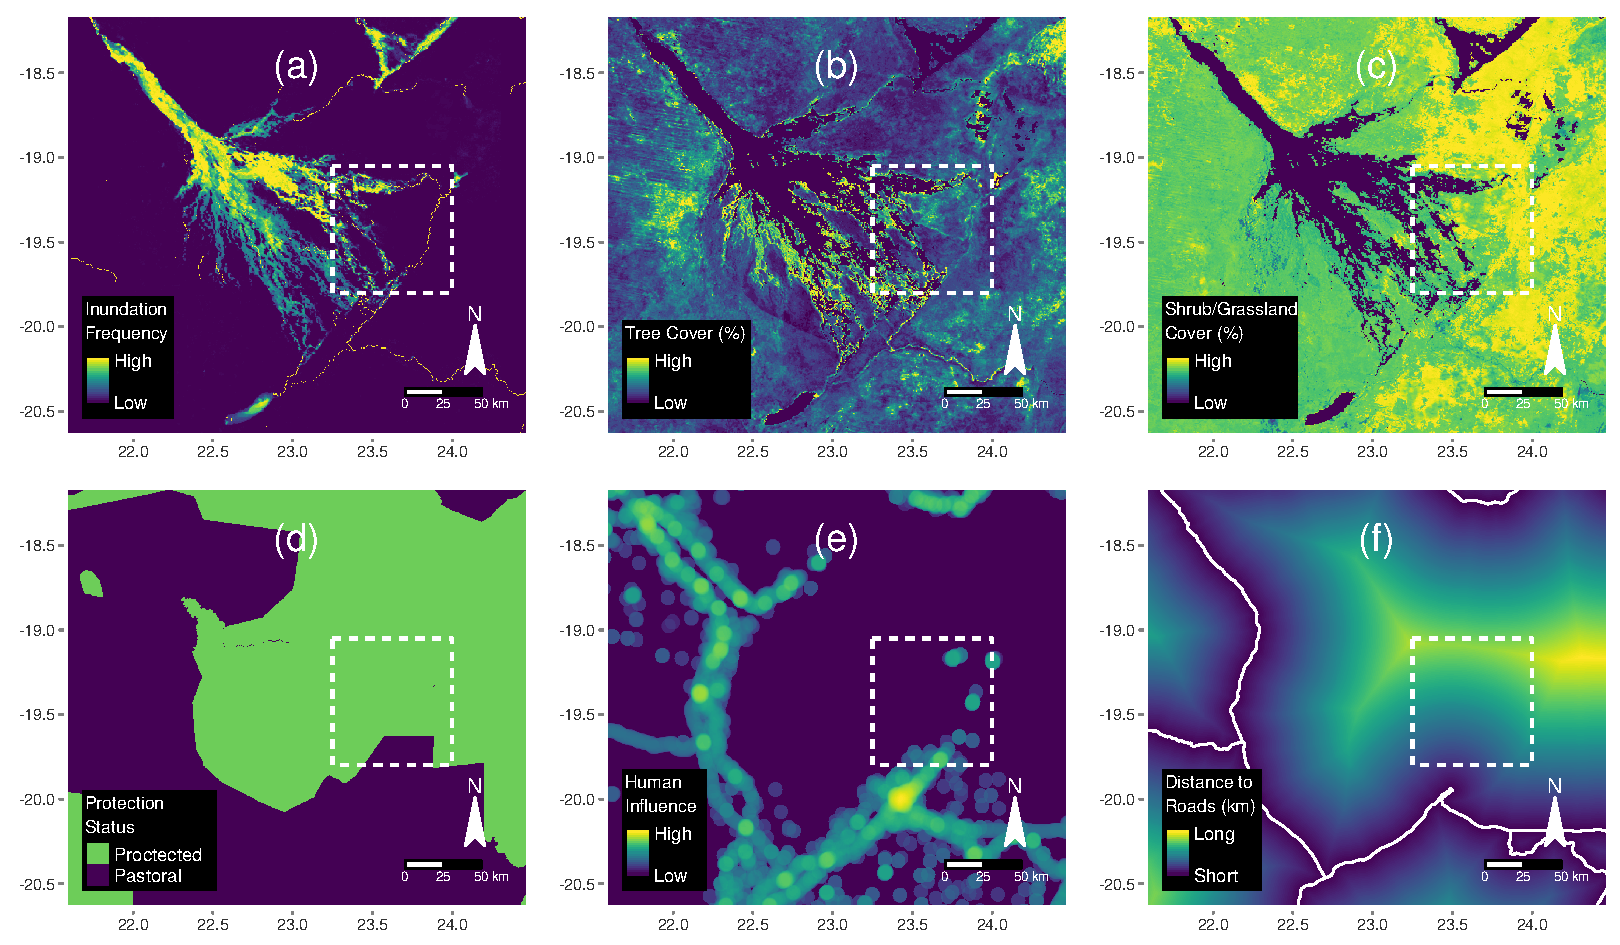
\includegraphics[width = \textwidth]{99_Covariates.pdf}
    \caption{Overview of covariates that we used in our models. Although all
    covariates were prepared for the extended study area, we present only an
    extract to maximize visibility. The white rectangle in each plot depicts our
    core study area. (a) Averaged layer of all binary maps of water and dryland
    that we acquired using our floodmapping algorithm. (b) Percentage cover of
    trees. (c) Percentage cover of shrubs/grassland. Note that anything not
    covered by trees or shrubs/grassland was deemed to be bare land. (d)
    Protection status of the area. (e) Human influence proxy, taking into
    account human density, farms, and roads. (f) Distance to nearest road (white
    lines depict actual roads).}
    \label{Covariates}
  \end{center}
\end{figure}

\newpage
\subsubsection{Land Cover}
% Overview
Land cover was represented by four layers: a binary layer distinguishing water
and dryland, and three continuous layers showing the percentage cover by
different vegetation types, combined adding up to 100\%.

% Water Layers
Water included open waters, rivers, wetlands, and swamps, whereas anything else
was presumed to be dryland. Because the flood extent of the Okavango Delta is
highly variable within and between years, we created weekly (8 days)
``floodmaps'', following the algorithm developed in \cite{Wolski.2017}. The
algorithm uses thresholding of SWIR reflectances of MODIS Terra satellite
imagery (MCD43A4, \cite{Schaaf.2015}) to separate water and dryland. As we
rewrote and slightly amended the original Python code in R, we describe the
underlying principles and indicate the discrepancies to the original algorithm
in \Cref{Appendix:FloodmappingAlgorithm}. While water in the Okavango Delta was
mapped dynamically, we used a static watermap for its surroundings. This static
map was based on Globeland's land cover dataset \citep{Chen.2015}, from which we
only retained the categories \textit{wetland} and \textit{water bodies} and
collectively reclassified them to \textit{water}. Globeland had an original
resolution of 30m x 30m, so we coarsened the layer to 250m x 250m using the mode
of each 250m x 250m cell. Lastly, we improved river representation using the
MERIT Hydro dataset \citep{Yamazaki.2019}, from which we added all rivers with a
width of over 10m to our floodmaps.

% Vegetation Layers
The three vegetation layers that we used in addition to the floodmaps were
derived from the MODIS Terra Vegetation Continuous Fields dataset (MOD44B,
\cite{Dimiceli.2015}). Combined, the three layers added up to 100\% and depicted
the percentage cover of tree-vegetation (henceforth trees), non-tree-vegetation
(henceforth shrubs/grassland), and non-vegetated (henceforth bare land). To
ensure that areas covered by the flood would get 0\% vegetation cover (i.e.
100\% bare land cover), we used our floodmap that aligned with the creation date
of the layers (30 March 2017) and manually defined pixels covered by the flood
as being 100\% bare land. The MODIS vegetation layers had a resolution of 250m x
250m, so we did not need to coarsen or interpolate them.

\subsubsection{Protection Status}
To assess whether dispersers preferred protected over unprotected (pastoral)
regions, we derived a binary layer separating the two categories. Corresponding
data on protection status was downloaded in shapefile format from the Peace
Parks Foundation \citep{PeaceParks.2019}. We simplified original categories to a
binary classification of protected and pastoral areas (see
\Cref{Reclassification} in \Cref{Appendix:Reclassification}). Protected areas
mainly included forest reserves, game reserves, wildlife management areas, and
NPs, whereas everything not covered by such categories was considered to be
pastoral area. Finally, we rasterized the two categories onto a binary raster (1
= protected, 0 = pastoral) with a resolution of 250m x 250m.

\subsubsection{Human Influence}
We defined human influence using a proxy that incorporated anthropogenic
pressures arising from (1) human density, (2) farming activities, and (3) roads.
Previous research revealed that veterinary fences have no influence on wild dog
movements \citep{Cozzi.2013b}, so we did not include them in our analysis.

% Human Density
(1) We obtained spatial human density estimates through Facebook's 30m x 30m
high-resolution population density dataset \citep{Facebook.2019}. The dataset
contained some human density that arose from lodges and other touristic
activities that we did not want to depict as human pressures, so we manually
removed such regions from the data. The resulting layer was coarsened to 250m x
250m by summing up human densities within 250m x 250m cells.

% Farming
(2) Information on farming activities was sourced from the Globeland
\citep{Chen.2015} and Cropland \citep{Xiong.2017} land cover datasets, from
which we only retained pixels that were classified as either \textit{cultivated
land} or \textit{croplands}. Both layers had a resolution of 30m x 30m and were
coarsened to 250m x 250m by summing up values within 250m x 250m cells. The
layers were then merged into a single binary layer depicting presence (= 1) or
absence (= 0) of farms within 250m x 250m cells.

% Roads
(3) Geo-referenced data on roads was downloaded in shapefile format from Open
Street Map \citep{OpenStreetMap.2019}. We omitted minor roads and only retained
main tar roads and trunks belonging to the biggest four categories (see
\Cref{RoadsDescription} in \Cref{Appendix:RoadCategories}). Finally, we
rasterized roads and trunks onto a binary raster (1 = roads, 0 = no roads) with
250m x 250m resolution.

To calculate a single proxy of human influence, we added up the layers
describing \textit{human density} (continuous), \textit{farming} (binary), and
\textit{roads} (binary). To reduce the influence of outliers, totaled values
were limited to a maximum of 50, which visually resulted in a good balance
between high and low anthropogenic influence and was therefore considered
appropriate for our analysis. To render the fact that humans influence their
surroundings beyond their presence, we followed \cite{Elliot.2014} and applied
to each pixel a 5 km spatial buffer within which we summed up and log-transformed
human-influence values.

\subsection{Habitat Selection Model}
\label{Modeling}
% Explanation of iSSF and Extraction
We used an integrated step selection function approach (iSSF, \cite{Avgar.2016})
to investigate dispersers' selection or avoidance for the above mentioned
spatial covariates. In the iSSF framework, covariates experienced along realized
steps are contrasted with covariates experienced along alternative random steps
that the animal could have taken, but decided not to. A step is here defined as
the connecting line between two consecutive GPS relocations
\citep{Turchin.1998}. In contrast to regular SSFs, iSSFs require to include
movement metrics as covariates in the corresponding conditional logistic
regression model. Their inclusion, in turn, allows simultaneous inference on
habitat and movement preferences, as well as to reduce potential biases in
estimated habitat preferences \citep{Forester.2009, Warton.2013, Avgar.2016}.

To conduct an iSSF analysis, we followed recommendations described in
Appendix S1 of \cite{Avgar.2016}. We prepared our GPS relocation data for
iSSF-analysis using the R-package \textit{amt} \citep{Amt.2019} and coerced
relocations recorded during dispersal to steps that were regularly spaced four
hours apart (allowing for a minor mismatch of up to 15 minutes). Steps that were
separated by more than four hours (e.g. due to GPS failure) were omitted from
further analysis. Each remaining step was paired with 24 random steps, generated
by sampling turning angles from a uniform distribution U(\(-\pi, \pi\)) and step
lengths from a gamma distribution that was fitted using realized step lengths
(shape = 0.3677, scale = 6,302)). Together, a realized and its 24 associated
random steps formed a stratum of 25 steps that received a unique identifier.

We extracted spatial covariates along realized and random steps as listed in
\Cref{ExtractedCovars}. For continuous covariates, we calculated the average
value, for binary covariates the percentage cover along the step. Since our
floodmaps were dynamic, we extracted values from the floodmap that was closest
in date to the actual step. We further derived a binary variable indicating
whether or not a step crossed a road and we identified the average distance of
each step to the nearest source of water or the nearest road. We square-rooted
the values for \textit{DistanceToRoads} and \textit{DistanceToWater} to render a
decreasing marginal impact of distance. We standardized extracted covariates to
a mean of zero and a standard deviation of one using a z-score transformation.
Furthermore, we screened covariates for correlation using Pearson's Correlation
Coefficient. None of the covariates were overly correlated (\(|r| > 0.6\),
\cite{Latham.2011}) and we retained all of them for modeling. To run a proper
iSSF analysis, we also included two movement metrics, namely the cosine of the
turning angle (\(cos(ta)\)) and the logarithm of the step length (\(log(sl)\)),
as covariates in our models \citep{Avgar.2016}. The movement metric \(cos(ta\))
served to describe the directionality of a step, as it transformed the circular
measure of (\(-\pi, +\pi\)) into a linear measure (-1, 1). Thus, positive values
indicated forward movements, whereas negative values indicated backward
movements \citep{Turchin.1998}. The movement metric \(log(sl\)), on the other
hand, was included as an indicator of the preferred step length. Since steps
were regularly spaced by four hours, \(log(sl\)) can also be interpreted as
movement rate.

\begin{table}[h]
  \begin{center}
    \caption{Overview of spatial covariates extracted along steps (see
    \Cref{Sources} in \Cref{Appendix:Sources} for an overview of the sources and
    resampling methods). *The covariates \textit{Water} and \textit{Dryland}
    added up to 100\%, which is why only \textit{Water} was included as
    explanatory variable in our models. The same applied for the group
    \textit{Shrubs/Grassland}, \textit{Trees}, and \textit{Bareland}, where we
    omitted \textit{Bareland} for modeling. Finally, from the group
    \textit{Protected} and \textit{Pastoral}, we only included
    \textit{Protected} in our models.}
    \label{ExtractedCovars}
    \resizebox{\textwidth}{!} {
      \begin{tabular}{lllll}
      \hline
      \textbf{Category} &
        \textbf{Covariate} &
          \textbf{Description} &
            \textbf{Values} \\
              % \textbf{Source(s)} \\
      \midrule
      \multirow{5}{*}{Land Cover}
        & Water
          & Percentage cover of water along step
            & 0-100\%\\
              % & \cite{Chen.2015}, \cite{Schaaf.2015}, \cite{Yamazaki.2019} \\
        & Dryland*
          & Percentage cover of dryland along step
            & 0-100\%\\
              % & Globeland, \cite{Schaaf.2015}, \cite{Yamazaki.2019} \\
        & DistanceToWater
          & Average distance of step to nearest water source
            & \(\geq\) 0m\\
              % & Globeland, \cite{Schaaf.2015}, \cite{Yamazaki.2019} \\
        & Shrubs/Grassland
          & Average non-tree vegetation along step
            & 0-100\%\\
              % & \cite{Dimiceli.2015} \\
        & Trees
          & Average tree-vegetation along step
            & 0-100\%\\
              % & \cite{Dimiceli.2015} \\
        & Bareland*
          & Average non-vegetated area along step
            & 0-100\%\\
              % & \cite{Dimiceli.2015} \\
      \hdashline
      \multirow{2}{*}{Protection Status}
        & Protected
          & Percentage cover of protected area along step
            & 0-100\%\\
              % & \cite{PeaceParks.2019} \\
        & Pastoral*
          & Percentage cover of unprotected area along step
            & 0-100\%\\
              % & \cite{PeaceParks.2019} \\
      \hdashline
      \multirow{3}{*}{Human Influence}
        & HumansBuffer5000
          & Average buffered (5 km) human influence along step
            & \(\geq\) 0\\
              % & \cite{Facebook.2019}, \cite{OpenStreetMap.2019}, \cite{Chen.2015}, \cite{Xiong.2017}\\
        & DistanceToRoads
          & Average distance of step to nearest road
            & \(\geq\) 0m\\
              % & \cite{Facebook.2019}, \cite{OpenStreetMap.2019}, \cite{Chen.2015}, \cite{Xiong.2017}\\
        & RoadCrossing
          & Binary value indicating whether a step crossed a road
            & 0, 1\\
              % & \cite{Facebook.2019}, \cite{OpenStreetMap.2019}, \cite{Chen.2015}, \cite{Xiong.2017}\\
      \hline
      \end{tabular}
    }
  \end{center}
\end{table}

% Permeability Model
\noindent We used the iSSF framework and parameterized a habitat selection model
that further served to predict landscape permeability. This habitat selection
model operated under the assumption that dispersing wild dogs assigned a
selection score \(w(x)\) of the following exponential form to each realized and
random step:

\begin{equation}
\label{EQ2}
  w(x) = exp(\beta_1 x_1 + \beta_2 x_2 + ... + \beta_n x_n)
\end{equation}

\noindent That is, the selection score \(w(x)\) of a step depended on its
associated covariates (\(x_1, x_2, ..., x_n\)), as well as on the animal's
preferences for these covariates (\(\beta_1, \beta_2, ..., \beta_n\)). The
probability that a step \(i\) was realized \(P(Y_{i} = 1\)) was then contingent
on the step's selection score, as well as on the selection scores of all
alternative steps in the stratum:

\begin{equation}
\label{EQ3}
  P(Y_{i} = 1 | Y_{1} + Y_{2} + ... + Y_{i} = 1) =
  \frac{w(x_{i})}{w(x_{1}) + w(x_{2}) + ... + w(x_{i})}
\end{equation}

% Conditional Logistic Regression Model
\noindent Habitat and movement preferences of interest, i.e. the \(\beta\)'s,
were estimated by comparing realized (scored 1) and random (scored 0) steps in a
conditional logistic regression model \citep{Fortin.2005}. In this model,
positive \(\beta\)-coefficients indicate selection of a covariate, negative
\(\beta\)-coefficients avoidance of a covariate. Selected covariates thus
contribute positively to expected landscape permeability, whereas avoided
covariates contribute negatively to landscape permeability.

% Mixed Effects Conditional Logistic Regression Model
To deal with multiple individuals, we applied mixed effects conditional logistic
regression analysis following \cite{Muff.2019}. Their approach allowed to
include individuals for whom some covariates did not vary, as well as to model
random intercepts and slopes for each covariate. We implemented their method
using the R-package \textit{glmmTMB} \citep{Mollie.2017}, where we fixed the
variance of the random intercept to an artificially high value of
10\textsuperscript{12} (for an explanation, see \cite{Muff.2019}) and used
animal ID to model random intercepts and slopes.

% AIC Model Selection
We defined the movement metrics \(cos(ta)\) and \(log(sl)\) as core covariates
and ran forward model selection based on Akaike's Information Criterion (AIC,
\cite{Burnham.2002}) for all other spatial covariates. That is, we started with
a basic model and iteratively increased model complexity upon reaching a
full model. We then ranked models according to AIC, assessed relative model
weights, and identified the most parsimonious model. Due to convergence issues,
we were unable to model interactions between spatial covariates.

% Validation
To validate the predictive power of the most parsimonious selection model, we
ran k-fold cross-validation for case-control studies as described in
\cite{Fortin.2009}. Using 80\% of randomly selected strata, we parameterized a
selection model and predicted selection scores \(w(x)\) for all steps in the
remaining 20\% of strata. According to predicted selection scores we assigned
ranks 1-25 within each stratum, with rank 1 indicating the highest selection
score. We identified the realized step's rank in each stratum and tallied rank
frequencies of realized steps across all strata. Finally, we carried out a
Spearman-rank correlation analysis between ranks and associated frequencies and
we recorded the correlation coefficient (\(r_{s, realized}\)). We repeated this
procedure 100 times with replacement and computed the mean correlation
coefficient (\(\bar{r}_{s, realized}\)), as well as its 95\% confidence
interval. For comparison, we also repeated the same procedure 100 times assuming
completely randomized preferences. We implemented randomized preferences by
omitting the realized step from each stratum and identifying the rank of a
randomly chosen random step within each stratum (now only ranks 1-24). Again, we
calculated Spearman's rank correlation coefficient (\(r_{s, random}\)), its mean
across repetitions (\(\bar{r}_{s, random}\)), and its 95\% confidence interval.
Ultimately, the validation proofed a significant prediction in case the
confidence intervals of \(\bar{r}_{s, realized}\) and \(\bar{r}_{s, random}\)
did not overlap.

\subsection{Permeability Surface}
We used the most parsimonious selection model and applied \Cref{EQ2} to predict
a permeability surface over the entire extent of the KAZA-TFCA. In other words,
we calculated the selection score \(w(x)\) for each 250m x 250m pixel covering
the extended study area given the pixel's spatial covariates. Note that the
movement metrics, i.e. \(cos(ta)\) and \(log(sl)\), did not enter the prediction
of landscape permeability as their inclusion in our habitat selection model
solely served to reduce the bias in estimated habitat preferences. By definition
of permeability, high selection scores resulted in high permeability, whereas
low selection scores resulted in low permeability. To reduce the influence of
outliers in predicted scores, we followed \cite{Squires.2013} and curtailed
predicted scores between the 1\textsuperscript{st} and 99\textsuperscript{th}
percentile of their original values. To predict permeability in the first place,
we needed to collapse all dynamic watermaps into a single layer, which we
achieved by identifying areas that were inundated in at least a quarter of all
our floodmaps. In order to be able to compare permeability across different
regions, we rescaled the permeability surface to a range between 0 and 1 using
\(f(x) = \frac{x - min(x)}{max(x) - min(x)}\). The most impermeable landscape
thus received a value of 0, whereas the most permeable landscape received a
value of 1.

\subsection{Least-Cost Paths \& Least-Cost Corridors}
To identify movement corridors within the extent of KAZA-TFCA, we calculated
least-cost paths (LCPs) and least-cost corridors (LCCs) between selected points
located in protected areas of our extended study area \citep{Adriaensen.2003,
Sawyer.2011}. Selected points were generated by overlaying the study area with a
regular grid of points, equally spaced 100 km apart and located within protected
areas that contiguously covered at least 700 km\textsuperscript{2}. The
threshold of 700 km\textsuperscript{2} was based on home-range requirements of
African wild dogs reported in \cite{Pomilia.2015} and served to eliminate
locations that were assumed unsuitable for supporting viable wild dog
populations. Finally, we defined centroids as source points for those protected
areas larger than 700 km\textsuperscript{2} that did not get any source points
from the regular grid. In total, we generated 68 points, which resulted in 2,278
unique pairwise combinations and therefore 2,278 unique LCPs and LCCs.

LCP analysis between source points was implemented using the R-package
\textit{gdistance} \citep{vanEtten.2018}. The package translated the (unscaled)
permeability surface into a network of nodes and used graph theory, in
particular Dijkstra's algorithm \citep{Dijkstra.1959}, to find shortest
effective distances between source points based on costs of moving from cell to
cell. The package thus required to convert the permeability surface to a
transition layer, where permeability values were translated into transition
probabilities for moving from one cell to another. In our case, the transition
probability of moving between two adjacent cells depended on their averaged
permeability. We allowed individuals to move from each cell to the cell's 8
surrounding neighbors (i.e. Moores neighborhood) and applied a geographic
correction to account for the fact that diagonal neighbors were more remote than
orthogonal neighbors. Because African wild dogs have been observed to cover
massive dispersal distances (\citeauthor{DaviesMostert.2012}, 2012;
\citeauthor{Masenga.2016}, 2016; \citeauthor{Cozzi.2020}, unpublished), we did
not limit LCPs to a maximal effective cost. After computation, we tallied
overlapping LCPs to identify high-frequency routes.

LCPs are often criticized because they identify single-pixel-wide paths and thus
obliterate potential alternative routes with only marginally higher costs
\citep{Pinto.2009}. Moreover, they implicitly assume that dispersers have
complete knowledge of the landscape and associated movement costs and therefore
always move along the least-costly route \citep{Carroll.2012}. Yet, individuals
rarely use a single optimum path, so that LCPs are often of limited biological
relevance \citep{Pinto.2009, Pullinger.2010}. To address these shortcomings, we
also calculated LCCs \citep{Pinto.2009, Sawyer.2011}, again using the R-package
\textit{gdistance}. In contrast to LCPs, LCCs overcome the
single-pixel-width-issue and reveal additional, slightly suboptimal dispersal
routes. To identify LCCs, we first computed for each source point a cumulative
cost map (see \Cref{LCCExample}), which indicated the total minimal costs
required to get from the selected point to any other location on the map. An LCC
between two points was then obtained by adding up their cumulative cost maps and
masking out all cell-values exceeding the lowest cell-value by more than 5\%. We
repeated this procedure for each possible pairwise combination of source points
and thereby identified LCCs between all 68 selected points. The resulting
corridor-maps were normalized to a range from zero to one using \(f(x) = \frac{x
- min(x)}{max(x) - min(x)}\) and totaled up into a single connectivity map.

% \begin{figure}[hbtp]
%   \begin{center}
%     \begin{tikzpicture}
%         \node[anchor=south west,inner sep=0] (image) at (0,0,0) {
%           \begin{minipage}{0.54\textwidth}
%             \begin{center}
%               \includegraphics[width = 0.5\textwidth]
%                 {99_LeastCostPaths(Example1).pdf}\\
%               \includegraphics[width = 1.0\textwidth]
%                 {99_LeastCostPaths(Example2).pdf}\\
%             \end{center}
%           \end{minipage}
%         };
%         \begin{scope}[x={(image.south east)},y={(image.north west)}]
%            %  % next four lines will help you to locate the point needed by
%            %  % forming a grid. comment these four lines in the final picture.↓
%            % \draw[help lines,xstep=.1,ystep=.1] (0,0) grid (1,1);
%            % \draw[help lines,xstep=.05,ystep=.05] (0,0) grid (1,1);
%            % \foreach \x in {0,1,...,9} { \node [anchor=north] at (\x/10,0) {0.\x}; }
%            % \foreach \y in {0,1,...,9} { \node [anchor=east] at (0,\y/10) {0.\y};}
%            %  % upto here
%             % \draw[black, line width = 0.5pt] (0.389, 0.627) -- (0.080, 0.477);
%             % \draw[black, line width = 0.5pt] (0.582, 0.627) -- (0.980, 0.477);
%             % \draw[white, line width = 1pt] (0.675, 0.290) -- (0.720, 0.265);
%             % \draw[white, line width = 1pt] (0.840, 0.255) -- (0.800, 0.260);
%             % \draw[white, line width = 1pt] (0.807, 0.205) -- (0.752, 0.205);
%         \end{scope}
%     \end{tikzpicture}
%     \caption{Figures illustrating the process of identifying a least-cost
%     corridor between the source points A and B. (a) Example of a permeability
%     surface, which serves to determine the costs of movement. (b1) Cumulative
%     cost map for point A, depicting the total minimal costs necessary to get
%     from point A to every other location. (b2) Cumulative cost map for point B,
%     depicting the total minimal costs necessary to get from point B to every
%     other location. (c) Summed cost maps of points A and B. (d) Masked out
%     corridor containing pixels that do not exceed the cheapest pixel by more
%     than 5\%.}
%     \label{LCCExample}
%   \end{center}
% \end{figure}

\begin{figure}[hbtp]
  \begin{center}
  \begin{minipage}{.25\linewidth}
    \begin{subfigure}[t]{.9\linewidth}
        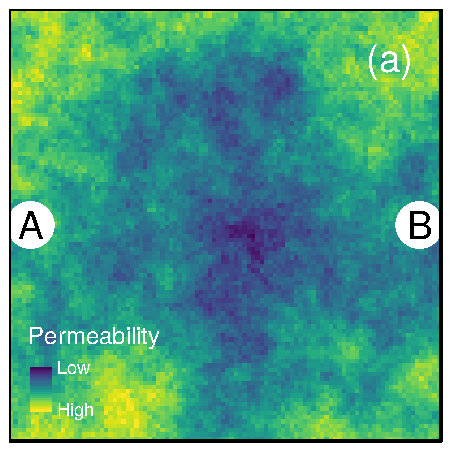
\includegraphics[width=\textwidth]{99_LeastCostPaths(Example1).pdf}
    \end{subfigure}
  \end{minipage}
  \begin{minipage}{.25\linewidth}
    \begin{subfigure}[t]{.9\linewidth}
        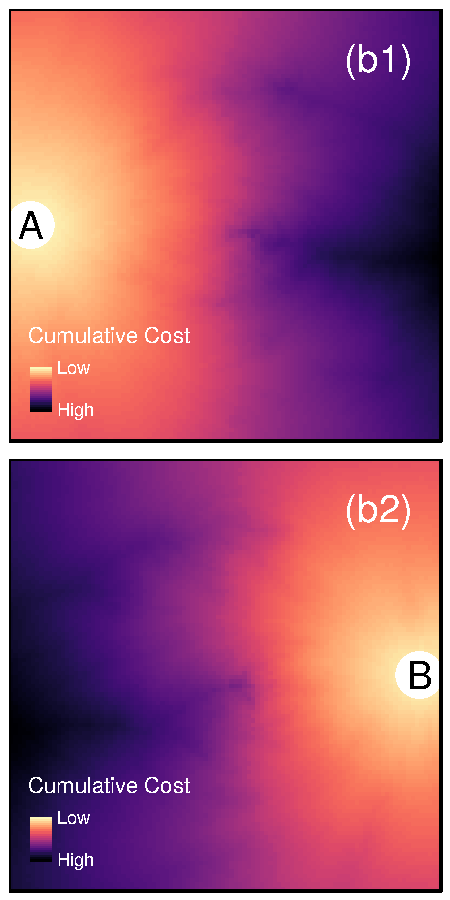
\includegraphics[width=\textwidth]{99_LeastCostPaths(Example2).pdf}
    \end{subfigure}
  \end{minipage}
  \begin{minipage}{.25\linewidth}
    \begin{subfigure}[t]{.9\linewidth}
        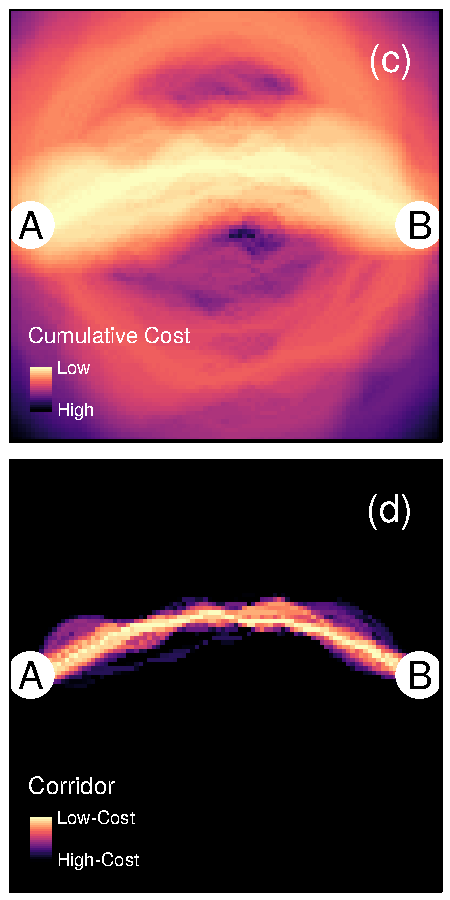
\includegraphics[width=\textwidth]{99_LeastCostPaths(Example3).pdf}
    \end{subfigure}
  \end{minipage}
  \caption{Figures illustrating the process of identifying a least-cost corridor
  between source points A and B following \cite{Pinto.2009}. (a) Example of a
  permeability surface, which determines the costs of movement. (b1) Cumulative
  cost map for point A, depicting the total minimal costs necessary to get from
  point A to every other location. (b2) Cumulative cost map for point B,
  depicting the total minimal costs to get from point B to every other location.
  (c) Summed cost maps of points A and B. (d) Masked out corridor containing
  pixels that do not exceed the cheapest pixel by more than 5\%.}
  \label{LCCExample}
  \end{center}
\end{figure}

\newpage
\section{Results}
\subsection{Habitat Selection Model}
Our most parsimonious habitat selection model (\(\Delta AIC > 2\) than any
alternative model; see \Cref{ModelAICs} in \Cref{AICs}) retained the covariates
\textit{Water}, \textit{DistanceToWater}, \textit{Trees},
\textit{Shrubs/Grassland}, \textit{HumansBuff5000}, and the fixed covariates
\(cos(ta)\) and \(log(sl)\) (\Cref{PermeabilityResults}a). Parameter estimates
showed that dispersing wild dogs moved in a directional and fast manner, as
indicated by selection of small turning angles, i.e. high \(cos(ta)\) (\(\beta\)
= 0.14; 95\% CI = 0.07 to 0.21, \Cref{PermeabilityResults}a) and long steps,
i.e. high \(log(sl)\) (\(\beta\) = 0.05, 95\% CI = 0.02 to 0.09,
\Cref{PermeabilityResults}a). Given the chance, dispersers avoided moving
through water (\(\beta\) = -0.5, 95\% CI -0.67 to -0.32,
\Cref{PermeabilityResults}a) but selected for locations in its vicinity,
although the effect was not significant (\(\beta\) = -0.24, 95\% CI = -0.67 to
0.19, \Cref{PermeabilityResults}a). Dispersers avoided areas that were densely
covered by trees (\(\beta\) = -0.18, CI = -0.32 to -0.04,
\Cref{PermeabilityResults}a) and preferred areas covered by shrubs/grassland
(\(\beta\) = 0.40, 95\% CI = 0.24 to 0.56, \Cref{PermeabilityResults}a).
Finally, dispersers avoided areas that were influenced by human presence and
activities (\(\beta\) = -0.47, 95\% CI = -0.87 to -0.07,
\Cref{PermeabilityResults}a).

\begin{figure}[h]
  \begin{center}
    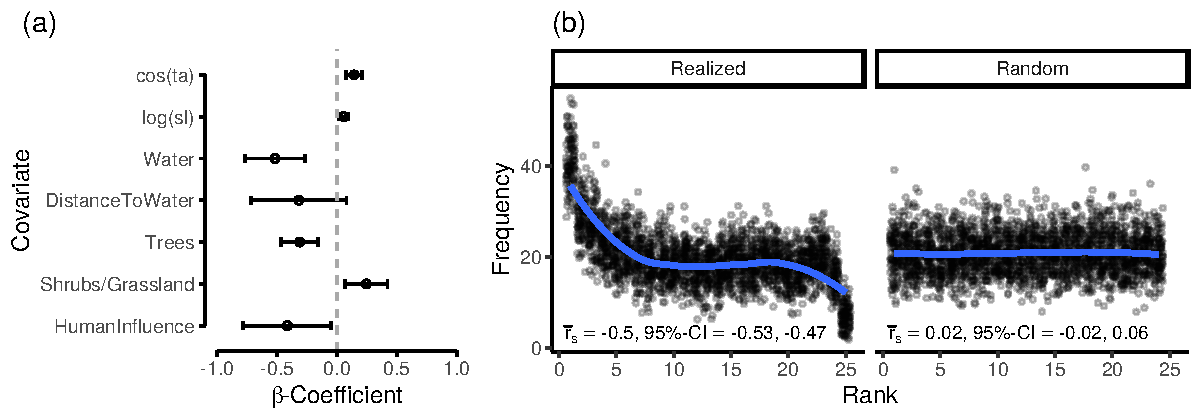
\includegraphics[width = \textwidth]{99_PermeabilityResults.pdf}
    \caption{(a) Estimated selection coefficients from the most parsimonious
    habitat selection model. Negative coefficients indicate avoidance of a
    covariate, positive coefficients selection of a covariate. Whiskers
    delineate the 95\%-CIs for estimated parameters. The intercept is
    meaningless in the iSSF framework and was thus omitted. (b) Results from the
    k-fold cross validation for case-control studies. The left graph shows rank
    frequencies of \textit{realized} steps according to predictions, whereas the
    right graph shows rank frequencies of \textit{randomly selected} steps
    according to predictions. \(\bar{r}_s\) indicates the mean correlation
    coefficient resulting from 100 repetitions of the k-fold cross validation.
    The blue smoothing line was fitted using a LOESS regression and solely
    serves to aid the eye in detecting the trends. Correlation coefficients
    suggest that our prediction is significant and robust, evidenced by the fact
    that the confidence intervals of \(\bar{r}_{s, realized}\) and \(\bar{r}_{s,
    random}\) do not overlap and that there is strong and significant
    correlation between ranks and associated frequency for realized steps.}
    \label{PermeabilityResults}
  \end{center}
\end{figure}

\newpage
\noindent Results from the k-fold cross-validation suggested that our prediction
was significant and robust, as highlighted by the fact that the 95\%-CIs
intervals of \(\bar{r}_{s, realized}\) (-0.45, CI = -0.48 to -0.42) and
\(\bar{r}_{s, random}\) (0.04, CI = 0.01 to 0.08) did not overlap
(\Cref{PermeabilityResults}b). Likewise, the significant correlation between
ranks and corresponding frequencies for realized steps suggested a good fit
between predictions and observations.

\subsection{Permeability Surface}
Our prediction revealed substantial differences in predicted permeability across
the entire study area (\Cref{PermeabilityMap}). Comparisons of median (Mdn)
permeability values (\Cref{PermeabilityComp}) showed that permeability inside
the boundaries of the KAZA-TFCA (Mdn = 0.21) was three times as high as
permeability outside it (Mdn = 0.07). A comparison across countries
(\Cref{PermeabilityComp}) showed that Angola (Mdn = 0.29) and Botswana (Mdn =
0.25) were characterized by comparably highly permeable landscapes, whereas
Zimbabwe (Mdn = 0.05) and Zambia (Mdn = 0.04) were relatively impermeable.
Namibia (Mdn = 0.16) ranged somewhere in between the two extremes. Across all
countries, protected areas provided higher permeability (Mdn = 0.21) than
human-dominated landscapes (Mdn = 0.07). A visual assessment of our permeability
surface revealed that northern Botswana had the highest density of permeable
landscapes (\Cref{PermeabilityMap}, bright yellow colors), despite the waters
of the Okavango Delta and Linyanti Swamp themselves provided highly impermeable
landscapes (\Cref{PermeabilityMap}, dark blue colors).

% \newgeometry{left=30mm,right=30mm,top=0mm,bottom=20mm}
% \begin{figure}[hbtp]
%   \begin{center}
%     \begin{tikzpicture}
%         \node[anchor=south west,inner sep=0] (image) at (0,0,0) {
%           \begin{minipage}{0.95\textwidth}
%             \includegraphics[width = \textwidth]{99_PermeabilityMap.pdf}
%             \includegraphics[width = \textwidth]{99_PermeabilityMap2.pdf}
%           \end{minipage}
%         };
%         \begin{scope}[x={(image.south east)},y={(image.north west)}]
%            %  % next four lines will help you to locate the point needed by
%            %  % forming a grid. comment these four lines in the final picture.↓
%            % \draw[help lines,xstep=.1,ystep=.1] (0,0) grid (1,1);
%            % \draw[help lines,xstep=.05,ystep=.05] (0,0) grid (1,1);
%            % \foreach \x in {0,1,...,9} { \node [anchor=north] at (\x/10,0) {0.\x}; }
%            % \foreach \y in {0,1,...,9} { \node [anchor=east] at (0,\y/10) {0.\y};}
%            %  % upto here
%             \draw[black, line width = 1pt] (0.389, 0.627) -- (0.080, 0.477);
%             \draw[black, line width = 1pt] (0.582, 0.627) -- (0.980, 0.477);
%             \draw[white, line width = 1pt] (0.675, 0.290) -- (0.720, 0.265);
%             \draw[white, line width = 1pt] (0.840, 0.255) -- (0.800, 0.260);
%             \draw[white, line width = 1pt] (0.807, 0.205) -- (0.752, 0.205);
%         \end{scope}
%     \end{tikzpicture}
%     \caption{(a) Predicted permeability surface for the extent of the KAZA-TFCA.
%     Permability was predicted by calculating selection scores \(w(x)\) for each
%     pixel based on the pixel's underlying covariates. Areas that dispersers find
%     easy to traverse are depicted in bright colors. Bold white lines delineate
%     the borders of the KAZA-TFCA, whereas dashed white lines show country
%     borders. (b) Detailed view of the Okavango Delta and Linyanti Swamp region,
%     which appears to provide the most suitable landscape for dispersers. The
%     white square highlights the core study area.}
%     \label{PermeabilityMap}
%   \end{center}
% \end{figure}
% \restoregeometry

% \newgeometry{left=30mm,right=30mm,top=0mm,bottom=20mm}
\begin{figure}[hbtp]
  \begin{center}
    \begin{tikzpicture}
        \node[anchor=south west,inner sep=0] (image) at (0,0,0) {
          \begin{minipage}{0.65\textwidth}
            \includegraphics[width = \textwidth]{99_PermeabilityMap.pdf}
          \end{minipage}
        };
        \begin{scope}[x={(image.south east)},y={(image.north west)}]
           %  % next four lines will help you to locate the point needed by
           %  % forming a grid. comment these four lines in the final picture.↓
           % \draw[help lines,xstep=.1,ystep=.1] (0,0) grid (1,1);
           % \draw[help lines,xstep=.05,ystep=.05] (0,0) grid (1,1);
           % \foreach \x in {0,1,...,9} { \node [anchor=north] at (\x/10,0) {0.\x}; }
           % \foreach \y in {0,1,...,9} { \node [anchor=east] at (0,\y/10) {0.\y};}
           %  % upto here
          % \node[text=white, circle, scale=1, font=\bfseries, inner sep = 0.5pt
          %   , draw=white] (No1) at (0.440, 0.350){1};
          % \node[text=white, circle, scale=1, font=\bfseries, inner sep = 0.5pt
          %   , draw=white] (No2) at (0.520, 0.438){2};
        \end{scope}
    \end{tikzpicture}
    \caption{Predicted permeability surface for the extent of the KAZA-TFCA.
    Permability was predicted by calculating selection scores \(w(x) =
    exp(\beta_1 x_1 + \beta_2 x_2 + ... + \beta_n x_n)\) for each pixel based on
    the pixel's underlying covariates (\(x_i\)) and estimated habitat
    preferences (\(\beta_i\)). Areas that dispersers find easy to traverse are
    depicted in bright colors. Bold white lines delineate the borders of the
    KAZA-TFCA, whereas dashed white lines show country borders.}
    \label{PermeabilityMap}
  \end{center}
\end{figure}
% \restoregeometry

% \begin{table}[h]
%   \caption{Comparison of median permeability across countries, separated
%   according to areas within and outside the KAZA-TFCA, as well as within and
%   outside protected areas. High values indicate high permeability, whereas low
%   values correspond to low permeability.}
%   \label{PermeabilityComp}
%   \begin{center}
%     \resizebox{\textwidth}{!} {
%       \begin{tabular}{llllllllr}
%       & & \multicolumn{2}{c}{KAZA-TFCA} && \multicolumn{2}{c}{Protection Status} \\
%       \cline{3-4} \cline{6-7}
%       Country & & Inside & Outside & & Protected & Pastoral & & Overall \\
%       \hline
%       Angola & & 1.67 & 0.59 & & 1.67 & 0.60 & & 1.03 \\
%       Namibia & & 0.91 & 0.49 & & 0.98 & 0.44 & & 0.59 \\
%       Botswana & & 1.17 & 0.69 & & 1.37 & 0.62 & & 0.91 \\
%       Zimbabwe & & 0.25 & 0.18 & & 0.32 & 0.17 & & 0.19 \\
%       Zambia & & 0.26 & 0.12 & & 0.23 & 0.13 & & 0.15 \\
%       \hline
%       Overall & & 0.75 & 0.26 & & 0.74 & 0.27 & & 0.38 \\
%       \end{tabular}
%     }
%   \end{center}
% \end{table}

\begin{table}[h]
  \caption{Comparison of median permeability (interquantile range in brackets)
  across countries, separated according to areas within and outside the
  KAZA-TFCA, as well as within and outside formally protected areas. High values
  indicate high permeability, whereas low values correspond to low
  permeability.}
  \label{PermeabilityComp}
  \begin{center}
    \resizebox{0.9\textwidth}{!} {
      \begin{tabular}{llllllllr}
      & & \multicolumn{2}{c}{KAZA-TFCA} && \multicolumn{2}{c}{Protection Status} \\
      \cline{3-4} \cline{6-7}
      Country & & Inside & Outside & & Protected & Pastoral & & Overall \\
      \hline
      Angola & & 0.46 (0.42) & 0.18 (0.40) & & 0.46 (0.42) & 0.18 (0.40) & & 0.29 (0.45) \\
      Namibia & & 0.26 (0.39) & 0.13 (0.20) & & 0.27 (0.38) & 0.12 (0.16) & & 0.16 (0.31) \\
      Botswana & & 0.33 (0.38) & 0.19 (0.23) & & 0.38 (0.35) & 0.17 (0.23) & & 0.25 (0.33) \\
      Zimbabwe & & 0.06 (0.25) & 0.05 (0.04) & & 0.09 (0.26) & 0.04 (0.03) & & 0.05 (0.07) \\
      Zambia & & 0.07 (0.11) & 0.03 (0.05) & & 0.06 (0.11) & 0.03 (0.05) & & 0.04 (0.07) \\
      \hline
      Overall & & 0.21 (0.39) & 0.07 (0.18) & & 0.21 (0.39) & 0.07 (0.18) & & 0.11 (0.29) \\
      \end{tabular}
    }
  \end{center}
\end{table}

\subsection{Least-Cost Paths \& Least-Cost Corridors}
Because LCPs identify the cheapest set of pixels between two selected points,
they typically run along the center of LCCs and traverse the same regions. The
two methods thus essentially return very similar information, but we show both
for the sake of clarity and comparison and because LCPs help more precisely
identifying discrete corridors. Our analysis revealed three major corridors
(\Cref{LeastCost}): one runs SE-NW and connects the Okavango-Linyanti ecosystem
in Botswana with Luengue-Luiana NP in Angola. One runs W-E between Chobe NP in
Botswana and Zimbabwe’s Hwange NP. One runs NE-SW, completely across unprotected
areas, and connects Kafue NP in Zambia with more central regions of the
KAZA-TFCA. With 637 LCPs passing through it, the Okavango-Linyanti region is the
highest frequented corridor. Several minor routes branch off these three major
corridors; this includes a southward connection between the Okavango-Linyanti
and the Central Kalahari Game Reserve, a southwesterly corridor connecting
Luengue-Luiana NP with Namibia’s Kaudom NP, and a northeasterly extension of the
Hwange corridor into Zimbabwe’s Matusadona NP. Our model did not detect any
significant direct corridors between Zimbabwe and Zambia and only a very limited
W-E direct connection between the Okavango region and Namibia’s Khaudum NP. We
also found little to no direct connectivity between peripheral points; that is,
most paths and corridors connecting two adjacent peripheral points run through
more central regions before heading towards their destination at the periphery.
Except for the Central Kalahari Game Reserve corridor, our model did not detect
any significant connectivity outside the boundaries of KAZA-TFCA.

\newgeometry{left=30mm,right=30mm,top=0mm,bottom=20mm}
\begin{figure}[hbtp]
  \begin{center}
    \begin{tikzpicture}
        \node[anchor=south west,inner sep=0] (image) at (0,0,0) {
          \begin{minipage}{0.95\textwidth}
            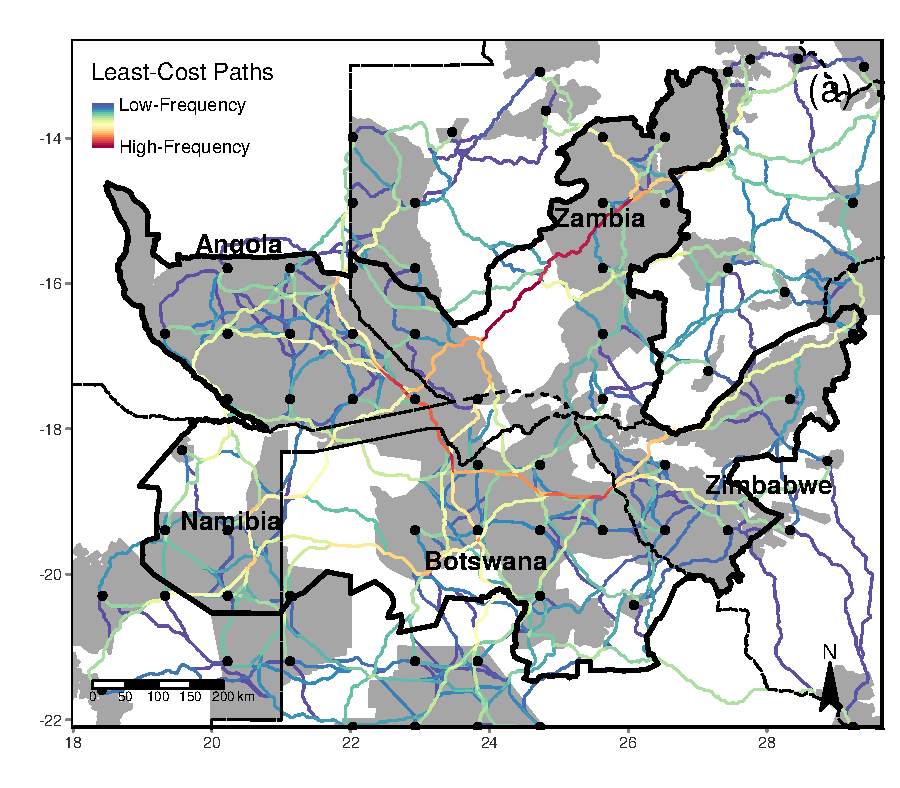
\includegraphics[width = \textwidth]{99_LeastCostPaths.pdf}
            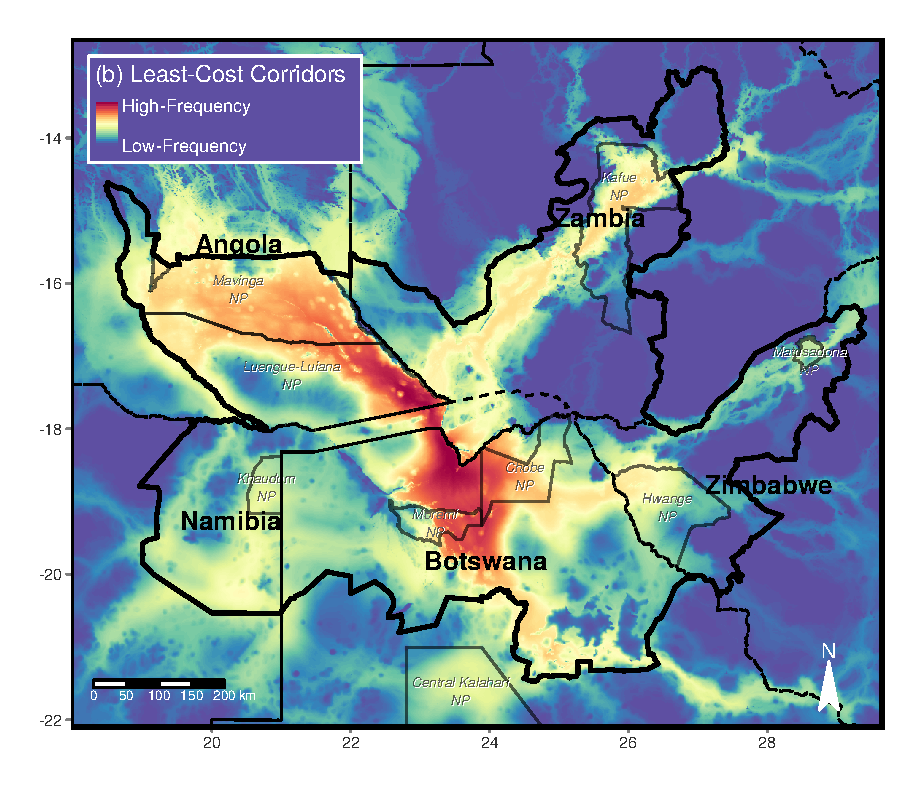
\includegraphics[width = \textwidth]{99_LeastCostCorrs.pdf}
          \end{minipage}
        };
        \begin{scope}[x={(image.south east)},y={(image.north west)}]
          % % next four lines will help you to locate the point needed by
          % % forming a grid. comment these four lines in the final picture.
          % \draw[help lines,xstep=.1,ystep=.1] (0,0) grid (1,1);
          % \draw[help lines,xstep=.05,ystep=.05] (0,0) grid (1,1);
          % \foreach \x in {0,1,...,9} {\node [anchor=north] at (\x/10,0) {0.\x};}
          % \foreach \y in {0,1,...,9} {\node [anchor=east] at (0,\y/10) {0.\y};}
          % % upto here
          % \node[text=black, circle, scale=1, font=\bfseries, inner sep = 0.5pt
          %   , draw=black] (No1) at (0.400, 0.700){1};
          % \node[text=black, circle, scale=1, font=\bfseries, inner sep = 0.5pt
          %   , draw=black] (No2) at (0.370, 0.760){2};
          % \node[text=black, circle, scale=1, font=\bfseries, inner sep = 0.5pt
          %   , draw=black] (No3) at (0.585, 0.780){3};
          % \node[text=black, circle, scale=1, font=\bfseries, inner sep = 0.5pt
          %   , draw=black] (No4) at (0.647, 0.697){4};
          % \node[text=black, circle, scale=1, font=\bfseries, inner sep = 0.5pt
          %   , draw=black] (No5) at (0.910, 0.770){5};
          % \node[text=black, circle, scale=1, font=\bfseries, inner sep = 0.5pt
          %   , draw=black] (No6) at (0.580, 0.658){6};
          % \node[text=black, circle, scale=1, font=\bfseries, inner sep = 0.5pt
          %   , draw=black] (No7) at (0.410, 0.640){7};
          % \node[text=black, circle, scale=1, font=\bfseries, inner sep = 0.5pt
          %   , draw=black] (No8) at (0.380, 0.665){8};
          % \draw[black, line width = 1pt, densely dotted] (No1) -- (0.500, 0.710);
          % \draw[black, line width = 1pt, densely dotted] (No2) -- (0.438, 0.760);
          % \draw[black, line width = 1pt, densely dotted] (No3) -- (0.565, 0.805);
          % \draw[black, line width = 1pt, densely dotted] (No4) -- (0.665, 0.685);
          % \draw[black, line width = 1pt, densely dotted] (No5) -- (0.885, 0.765);
          % \draw[black, line width = 1pt, densely dotted] (No6) -- (0.540, 0.650);
          % \draw[black, line width = 1pt, densely dotted] (No7) -- (0.450, 0.645);
          % \draw[black, line width = 1pt, densely dotted] (No8) -- (0.345, 0.690);
        \end{scope}
    \end{tikzpicture}
    \caption{(a) Source points (black dots) and corresponding least-cost paths
    leaving from protected areas (light grey). Note that only contiguous
    protected areas covering more than 700 km\textsuperscript{2} are depicted.
    Continuous thin black lines indicate the borders of the KAZA-TFCA, whereas
    dashed black lines delineate country-borders. (b) Least-cost corridors
    between the same source points as illustrated in subfigure (a). For ease of
    spatial reference we also labeled some national parks (dark-grey).}
    \label{LeastCost}
  \end{center}
\end{figure}
\restoregeometry

\newpage
\section{Discussion}
\label{Discussion}
% Recap of Study
We combined GPS relocation data of dispersing African wild dog coalitions with
spatial environmental and anthropogenic covariates to gain information on
habitat selection or avoidance during dispersal. We then used this knowledge to
create a permeability surface and assess connectivity by identifying dispersal
corridors across the world’s largest transboundary conservation area, the
Kavango-Zambezi Transfrontier Conservation Area.

\subsection{Habitat Selection Model}
% Finding: Human Influence
Our results indicate that dispersers avoided anthropogenic influences,
highlighting that human presence or activities constitute some of the main
obstacles to connectivity. While \cite{Masenga.2016} found similar avoidance of
human-dominated landscapes by dispersers in East Africa,
\cite{DaviesMostert.2012} reported a high willingness of dispersers to cross
such landscapes in South Africa. Our findings support the notion that dispersers
forgo human-dominated landscapes and we conjecture that differences to
observations by Davies-Mostert and colleagues are due to the unavailability of
alternative ``natural'' routes in South Africa. That is, dispersers in South
Africa may be forced to cross human-dominated landscapes despite a strong
aversion against human presence.

% Finding: Water
Water was identified as being another major obstacle to dispersal. According to
earlier studies, water is almost impermeable for resident packs and it is
assumed that residents use water bodies as easy-to-defend territory boundaries
\citep{Cozzi.2013}. Although dispersers have different needs and motivations
than residents, they have also been shown to be partially hindered by larger
water bodies (\citeauthor{Abrahms.2017}, 2017; \citeauthor{Cozzi.2020},
unpublished). Our findings thus align with previous research and stress the
importance to accurately and dynamically represent water bodies, notably for
such pulsing ecosystems as represented by the Okavango Delta.

% Finding: Distance To Water
While we found that dispersers avoided moving \textit{through} water, we
revealed a preference for moving \textit{close to} water. We hypothesize that
high prey-availability (e.g. impala) in proximity to water explains this result.
It is well documented that water is a major driver of wildlife and that it
determines the distribution of many herbivores, especially in dry biomes
\citep{Western.1975}. For the Okavango Delta, in particular, it has been shown
that prey abundance strongly correlates with the extent of the flood
\citep{Bonyongo.2005}. An increasing concentration of ungulates around remaining
water-sources during the dry season \citep{Ogutu.2014} therefore might attract
dispersing wild dogs. Following the same logic, however, apex predators (e.g.
lions, spotted hyenas) and resident wild dogs may also prefer proximity to water
\citep{Valeix.2009} and may occasionally force dispersing wild dogs to move
distant to water \citep{Ndaimani.2016} to avoid intraguild competition
\citep{Creel.1996, Mills.1997}. We could not control for the presence or absence
of apex predators or conspecifics during dispersal as we lacked corresponding
data, but these considerations might explain why we did not find a statistically
clear effect of distance to water.

\subsection{Permeability Surface}
% Finding: Permeabilities
According to our prediction of landscape permeability, northern Botswana and
southern Angola provide relatively permeable landscapes. High permeability in
these countries is mainly caused by a combination of low human presence and
activities, low tree cover, high shrubs/grassland cover and close distance to
water. Although swamps, wetlands, and permanent water provide little
permeability themselves, their surroundings act as strong attractants to
dispersers. The low permeability that characterizes Zambia and Zimbabwe, on the
other hand, is mainly caused by severe anthropogenic presence and other human
activities. Even though the KAZA-TFCA covers the majority of permeability
hot-spots, several highly permeable regions remain uncovered by the KAZA-TFCA,
offering exciting opportunities for future expansions of already existing
protected areas.

\subsection{Least-Cost Paths \& Least-Cost Corridors}
% Finding: Overlap Corridors and KAZA
Our analyses of dispersal paths and corridors suggest that all major dispersal
corridors of African wild dogs run within the boundaries of the KAZA-TFCA,
demonstrating the potential value of such an initiative. Within the KAZA-TFCA,
however, some key connectivity areas are not formally protected and their
protection status may be subject to future changes under the influences of an
expanding human population, farming, and cropping industry. Although overall
connectivity gradually decreases towards the borders of the study area, this
might partly be a result of boundary-effects \citep{Koen.2010}. In general, our
network of corridors shows high similarities to predicted movement corridors of
dispersing lions \citep{Elliot.2014}, which not only reinforces confidence in
our predictions but also suggests potential synergies between conservation of
the two species.

% Finding Regarding Dispersal Hub
Importantly, we identified the Okavango-Linyanti region as a potential dispersal
hub through which dispersers gain access to more peripheral regions of the
KAZA-TFCA. While this might partly be owed to the area's central position within
the KAZA-TFCA, it is likely also due to its environmental and anthropogenic
characteristics, namely due to the absence of human activities and the presence
of impermeable water bodies, such as the Okavango Delta and the Linyanti Swamp,
which potentially funnel dispersal movements. The region is also instrumental
for connecting subpopulations remaining in Zambia’s Kafue and Zimbabwe’s Hwange
NPs. These subpopulations are currently separated by the Zambezi River, forcing
dispersers to detour via northern Botswana to reach more peripheral areas. The
key role of the Okavango-Linyanti region for the overall connectivity of the
KATA-TFCA thus calls for actions to secure its protection status in the future.
While the region is presently a Wildlife Management Area devoted to photographic
tourism, it has neither the status of a National Park nor that of a Game Reserve
and so potentially faces growing pressure towards exploitation of its natural
resources.

% Finding: Corridor Between Moremi & Kafue
A similar case of non-formally protected but key dispersal landscape is
represented by the area south of Kafue NP in Zambia, for which disruption of its
main and narrow dispersal corridor would result in considerable isolation of its
subpopulations, for no other corridor links Kafue NP to the rest of the
KAZA-TFCA.

% Finding: Corridor Between Moremi & Kalahari
Our results also revealed a potential southwards corridor between the
Okavango-Linyanti ecosystem and the Central Kalahari Game Reserve.
\cite{Elliot.2014} identified a similar corridor for dispersing lions, which
shows that protecting the area would benefit lions and wild dogs alike. Some
areas through which the corridor runs are neither part of KAZA-TFCA nor of any
protected status. Human presence and activities along the national road that
longitudinally traverses the corridor may limit realized connectivity,
especially since the road is reported to increase wild dog mortality through
direct persecution and collisions (\citeauthor{Cozzi.2020}, unpublished). In
fact, despite having dispersed south of the Okavango Delta, none of the
monitored dispersing coalitions crossed the national road and reached the
Central Kalahari Game Reserve (\citeauthor{Cozzi.2020}, unpublished).

\subsection{Future Research}
% Future Research: Genetic Resistance
While we assessed landscape permeability purely based on GPS relocation
data, future studies could challenge and test our predictions using genetic data
\citep{Spear.2010}. Similar comparisons have been conducted for other species
and revealed a surprisingly high overlap between predicted landscape
permeability based on genetic and movement data \citep{Cushman.2010}. Genetic
data would also deepen our understanding of the degree to which subpopulations
admix and of the overall genetic diversity found in different subpopulations
\citep{Girman.2001}. Based on our connectivity network, we would expect to find
a low genetic diversity for populations that live in insufficiently connected
habitats, whereas populations residing at dispersal hotspots, such as the
Okavango-Linyanti ecosystem, should exhibit a relatively diverse gene-pool.

% Future Research: Better Covariates
Future research should also strive to improve the representation of
geo-referenced covariates. Because we predicted connectivity for such an
extensive area, we were strongly limited in available and reliable land cover
data. As a result, our representation of vegetation remained rather basic with
only three vegetation types (tree-cover, shrubs/grassland, bare land). Although
there are a few large-scale, high-resolution land cover datasets, such as
Globeland's 30m \citep{Chen.2015} and the European Space Agency's and 20m
\citep{ESA.2019} land cover datasets, we found their classifications often
erroneous for our study area. This is probably owed to the KAZA-TFCA's unique
landscape and corresponding difficulties in remote sensing satellite imagery
using traditional indices \citep{Wolski.2017}. Nevertheless, land cover is a
very powerful predictor of animal movement \citep{Thurfjell.2014}, highlighting
the need for more reliable land cover data.

% Future Research: Competitor Presence
Similarly, we would desire better knowledge of the whereabouts of other species.
In particular, we would desire location data of apex predators, prey, and
conspecifics. It is well documented that resident wild dogs frequently compete
with other carnivores \citep{Creel.1998} and we would expect to find competition
between dispersing wild dogs and apex predators too. Furthermore, knowledge
about the spatial distribution of prey could verify our hypothesis that
dispersers move along water due to prey-availability. Lastly, we could not
control for the likelihood of encountering conspecifics during dispersal. Yet,
for dispersing meerkats, a species with a surprisingly similar social structure
to wild dogs, it has been shown that the social landscape, i.e. the presence or
absence of conspecifics, strongly shapes behavior during dispersal
\citep{Cozzi.2018}. More specifically, it has been shown that dispersers select
for high density of conspecifics while still inside their home-range, but that
they avoid high densities of conspecifics once they leave their natal home-range
(we replicated this analysis for the core study area; see
\Cref{Appendix:SocialLandscape}). Spatially explicit knowledge about the
distribution of foreign wild dogs is thus desirable and would certainly deepen
our understanding of dispersal behavior. However, constructing meaningful and up
to date social landscapes is extremely challenging and requires vast amounts of
movement data, especially for such a wide-ranging species as the African wild
dog \citep{Pomilia.2015}.

% Future Research: Global Resistance Mapping
Besides urging for more and better data, we also want to emphasize that our
analytical approach is neither limited to African wild dogs nor our study area.
All covariates used throughout this study are available on a global scale and
they are likely to be important determinants of landscape permeability for other
species. Our framework could easily be applied to assess connectivity for a wide
range of species, provided suitable relocation data of the species exist.
Expanding our analyses to other species would surely yield interesting insights
on the congruence of movement corridors and thereby highlight areas that are
exceptionally valuable for the conservation of multiple species.

% Future Research: Simulating Dispersal
To this end, we identified movement corridors between pre-defined start and
end-points. This assumes that dispersers have a specific end-point in mind when
dispersing, which is likely not always the case. However, pre-defining
end-points might not even be necessary, as one could use the iSSF framework as a
mechanistic movement model to simulate dispersal without a known end-point. That
is, one could define a set of source points at locations where wild-dogs are
assumed or known to reside and simulate dispersers according to identified
habitat-preferences. As a consequence, movement corridors would emerge naturally
as the result of a myriad of simulated dispersal events (for an example of
simulated dispersal events see \Cref{Appendix:DispersalSimulation}).

\newpage
\subsection{Conclusion}
Our results demonstrate that the majority of dispersal corridors for African
wild dogs are covered by the boundaries of the KAZA-TFCA, suggesting that the
KAZA-TFCA will significantly contribute to the long-term viability of this
species. Nevertheless, some unprotected dispersal routes do exist outside the
KAZA-TFCA and indicate opportunities for further expansions in the future.
Moreover, our connectivity network of least-cost paths and least-cost corridors
revealed the Okavango-Linyanti region as a central dispersal hub through which
dispersers gain access to more remote regions of the KAZA-TFCA. Therefore, we
stress the importance of northern Botswana for the conservation of this
charismatic species. Finally, our investigations showed that human pressures
remain a severe impediment to dispersal and therefore reduce landscape
connectivity. Successful conservation of the African wild dog is thus contingent
on the willingness of local authorities, policymakers, and land managers to
preserve areas that are largely liberated from human strains. Ultimately, our
work contributes to the growing field of connectivity literature and has
important implications for the management and conservation of the endangered
African wild dog.

\newpage
\section{Acknowledgements}
All of this work would not have been possible without the aid of several helpful
people. I would first like to thank Prof. Arpat Ozgul, the leader and mastermind
of our research group, whose expertise in statistics, biological processes and
scientific writing was invaluable for my work. Moreover, I want to thank
Gabriele Cozzi for his excellent guidance, all the interesting discussions, his
constructive criticism, valuable revisions in the manuscript, and of course his
constant supply of freshly brewed coffee. Particular gratitude goes to Dominik
Behr, who supervised my work daily and greatly contributed to all aspects of the
thesis. I genuinely enjoyed the frequent meetings and brainstorms and I feel
privileged to have had the opportunity of working with such a great scientist. I
am also greatly indebted to Prof. John Fieberg, who visited our department this
summer and invested a great amount of time to consult and improve all
statistical aspects of the thesis, as well as to deepen my understanding of
movement ecology. Furthermore, I thank the Okavango Research Institute,
especially Piotr Wolski, for sharing all of their Python scripts, floodmaps, and
knowledge on developing dynamic floodmaps. Also, I want to thank Stefan Sommer
for sharing and teaching his hard-earned knowledge on scientific writing.
Additionally, I want to thank all of my colleague master students who have been
wonderful companions and made the time at university a blast. Likewise, I thank
my parents for supporting all of my undertakings and for providing first-class
shelter and food. Last, but most definitely not least, I also greatly thank my
girlfriend, who was always there for me and provided welcome distractions for my
mind.

\newpage
\begingroup
\singlespacing
\bibliography{Literatur}
\endgroup

\newpage
\appendix
\section{Appendix}
\subsection{Floodmapping Algorithm}
\label{Appendix:FloodmappingAlgorithm}
To implement the floodmapping algorithm, we defined two sets of polygons located
in the region of the Okavango Delta (see \Cref{Floodmapping}). The first set
consisted of areas known to be permanent dryland, whereas the second set
consisted of permanent waters. Since we were unable to retrieve the original
polygons used in \cite{Wolski.2017}, we geo-referenced one of their
illustrations and traced the polygons there. After recreation of the polygons,
we used the R-package \textit{getSpatialData} \citep{Schwalb.2018} to download
and pre-process all relatively cloud-free MODIS Terra images (MCD43A4,
\cite{Schaaf.2015}) available for the period of our dispersal events. Assessment
of cloud cover was based on visual inspection of MODIS images on ORI's website
\citep{ORI.2019}. The MCD43A4 MODIS product is particularly useful for dynamic
floodmapping because it is updated with new composite images every 8th day
\citep{Wolski.2017}. After download, we classified each MODIS image into a
binary map of water (flood) and dryland using a threshold that was identified as
follows. First, we extracted all reflectance values of MODIS Terra Band 7 within
the water- and dryland-polygons. Second, we computed histograms of
water-reflectances and dryland-reflectances and empirically verified that
reflectances of the two groups were sufficiently distinct. More specifically, we
checked if superimposing the two histograms resulted in a bimodal plot. This was
said to be achieved if the 99\textsuperscript{th} percentile of
water-reflectances did not severely exceed the 1\textsuperscript{st} percentile
of dryland-reflectances (\(p_{0.99, water} - \frac{10}{255} < p_{0.01,
dryland}\)). Third, if peaks were sufficiently different, we calculated a
threshold (\(t\)) using \Cref{EQ1}:

\begin{equation}
\label{EQ1}
t = \widetilde{p}_{water} + 0.3 * (\widetilde{p}_{dryland} -
\widetilde{p}_{water})
\end{equation}

\noindent where \(\widetilde{p}_{water}\) and \(\widetilde{p}_{dryland}\) were
the median reflectances of water and dryland, respectively. We then classified
all pixels of MODIS Terra Band 7 with a value greater than \(t\) as dryland and
all pixels with a value smaller than \(t\) as water.

\begin{figure}[h]
  \begin{center}
    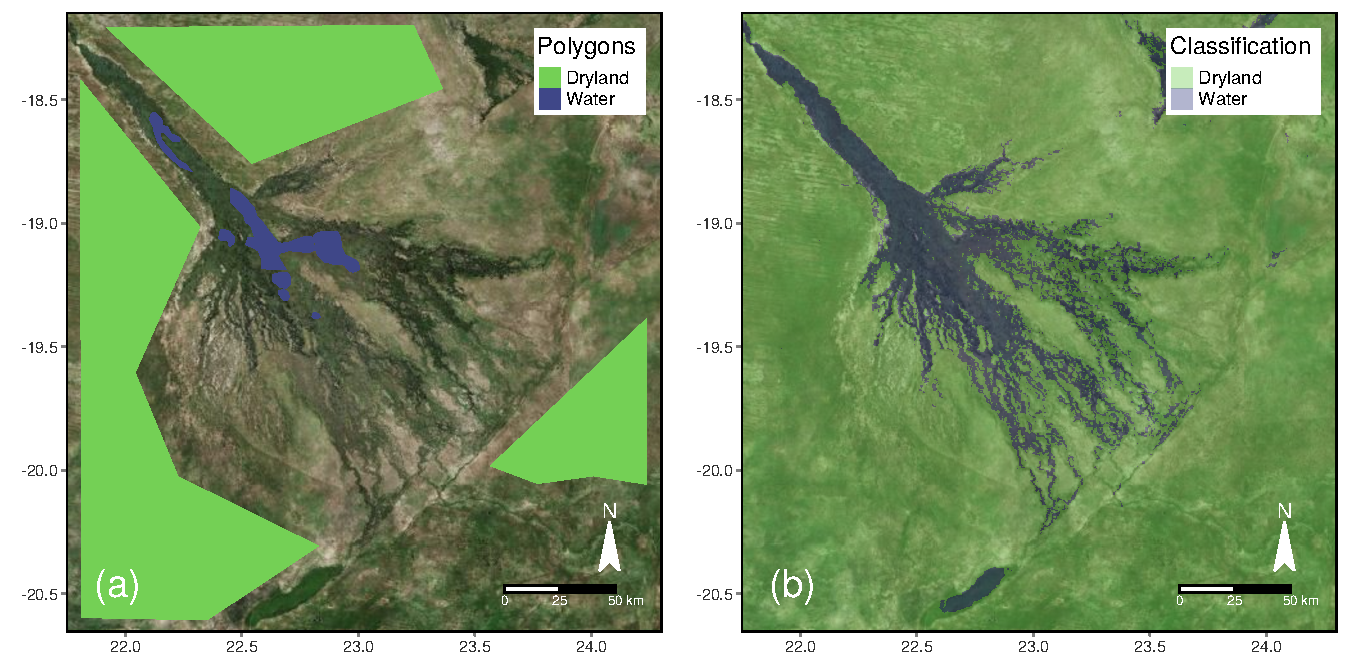
\includegraphics[width = \textwidth]{99_Floodmapping.pdf}
    \caption{Figures describing the floodmapping algorithm. (a) The colored
    polygons indicate permanent waters and permanent dryland. Below these
    polygons we extracted reflectance values of MODIS Terra Band 7 and used
    their repsective medians to calculate a classification threshold. (b)
    Example of a classified MODIS Terra Band 7 image after application of the
    threshold.}
    \label{Floodmapping}
  \end{center}
\end{figure}

% Dynamic Wetmask
Importantly, bimodality was not always achieved and in some cases no floodmap
could be calculated. In fact, it appears that non-bimodality caused the ORI
algorithm to fail since the end of 2018, such that no floodmaps have been
generated since then (ORI, personal comm.). We hypothesized that this was caused
by the application of static water-polygons that did not cover permanent waters
correctly anymore. Therefore, we revised the algorithm and allowed for a more
dynamic polygonization of water. That is, for each MODIS image we calculated new
water-polygons comprising areas that were covered by the flood in 99\% of the
floodmaps from the previous five years. All of the necessary floodmaps from
previous years were kindly provided to us by ORI. Using this slightly amended
approach, we were able to address some of the bimodality issues and to classify
several additional floodmaps for the period of our study. Because MODIS Terra
Band 7 had a resolution of 500m x 500m, we interpolated all maps to 250m x 250m.

% Validation
To validate and compare the performance of our own algorithm to the original
ORI-algorithm, we randomly sampled 48 dates for which ORI prepared classified
images. To make sure that months were equally represented in the sampled dates,
we employed stratified sampling based on months (regardless of the year) and
randomly sampled four maps for each month. For the sampled dates we downloaded
and classified MODIS Terra Band 7 images and compared our classified images to
those provided by ORI (\Cref{FloodmappingValidation}). For each pair of maps we
created a difference map indicating false positives and false negatives and
computed the relative number of wrongly classified pixels. We achieved an
overall accuracy of 97\%, which presumably is an underestimate of the true
performance, as we introduced some errors when resampling the ORI-maps to our
reference raster.

\begin{figure}[ht]
  \begin{center}
    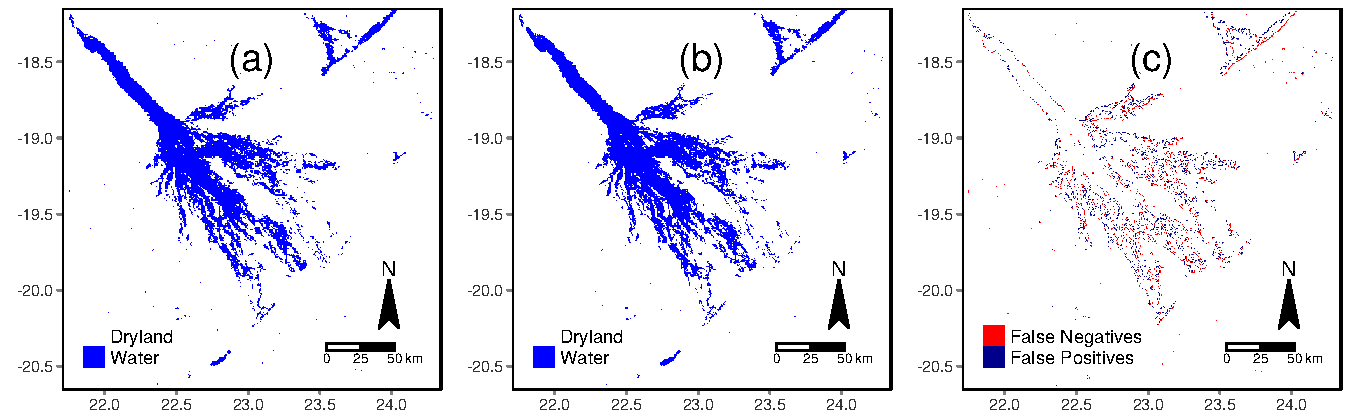
\includegraphics[width = \textwidth]{99_FloodmappingValidation.pdf}
    \caption{Validation procedure of our floodmapping algorithm. (a) Classified
    image that was provided to us by ORI. (b) Image for the same date but now
    classified using our own algorithm. (c) Difference image indicating false
    positives and false negatives in our own classification.}
    \label{FloodmappingValidation}
  \end{center}
\end{figure}

% Static Watermap
\noindent While water in the Okavango Delta was mapped dynamically, we used a
static watermap for its surroundings. This static map was based on Globeland's
land cover dataset \citep{Chen.2015}, which contains ten land cover categories.
From the original layer we only retained the categories \textit{wetland} and
\textit{water bodies} and collectively reclassified them to \textit{water}.
Globeland had an original resolution of 30m x 30m, so we coarsened the layer to
250m x 250m using the mode of each 250m x 250m cell. Lastly, we improved river
representation using the MERIT Hydro dataset \citep{Yamazaki.2019}, from which
we added all rivers with a width of over 10m to our watermaps. The entire
process resulted in several hundred watermaps, of which 72 represented the
closest watermap to one of our GPS relocations.

\begin{figure}[h]
  \begin{center}
    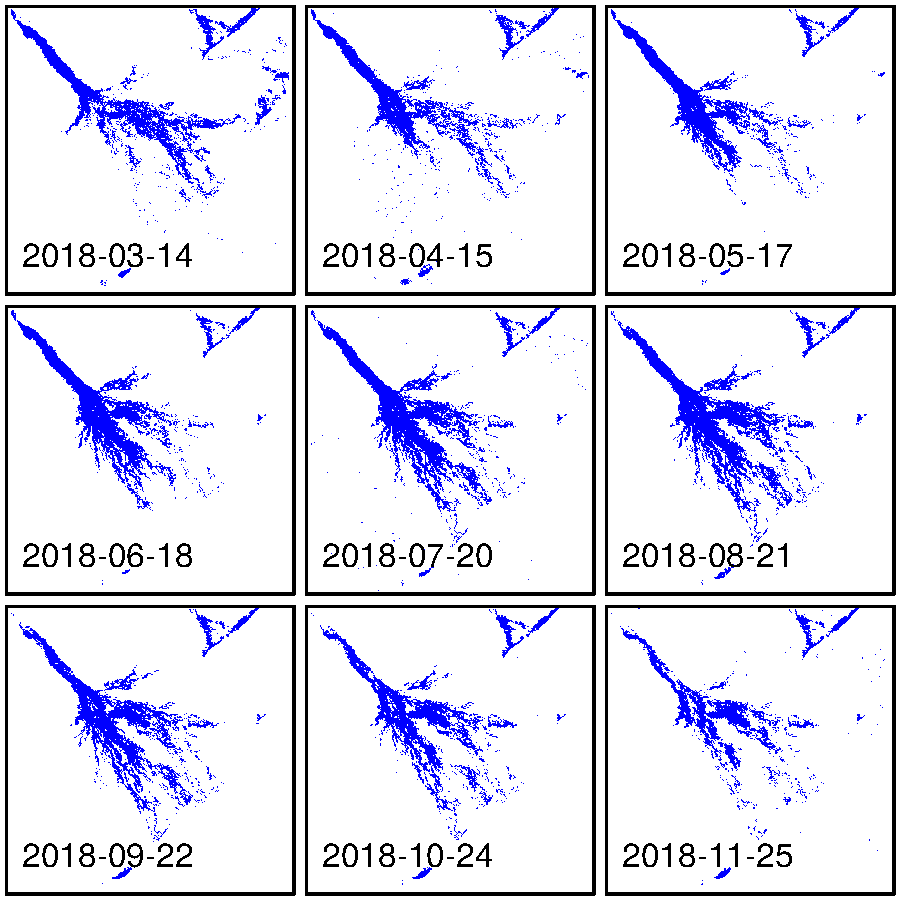
\includegraphics[width = \textwidth]{99_FloodPulse.pdf}
    \caption{Sequence of floodmaps showing a typical flood pulse throughout the
    year. The flood arrives from the north-western corner (so called
    ``pan-handle'') of the Okavango Delta and slowly descents through the delta
    in south-eastern direction, where it nourishes several tributaries. The
    extent of the flood peaks around August or September and then slowly
    retracts. Between December and March the reflectance properties of water and
    dryland change, which is why often no accurate floodmaps can be obtained for
    these months using remote sensing techniques.}
    \label{FloodPulse}
  \end{center}
\end{figure}

\newpage
\subsection{Reclassification of Protected Areas}
\label{Appendix:Reclassification}
\begin{table}[h]
  \caption{Reclassification of protected areas. Data on protection status was
  obtained from the \cite{PeaceParks.2019}. We simplified original categories to
  a binary classification of protected and unprotected (pastoral) areas. Any
  area that was not represented by one of the categories listed in
  \Cref{Reclassification} was deemed to be pastoral landscape.}
  \label{Reclassification}
  \begin{center}
    \resizebox{\textwidth}{!}{
      \begin{tabular}{llp{11cm}}
      \toprule
      \textbf{Original Category} &
        \textbf{Reclassification} &
          \textbf{Comment} \\
      \midrule
      Communal Conservancy &
        Protected &
          No comment\\
      Community Forest &
        Protected &
          No comment\\
      Conservancy &
        Protected &
          No comment\\
      Forest Reserve &
        Protected &
          No comment\\
      Game Management Area &
        Protected &
          No comment\\
      Game Park &
        Protected &
          No comment\\
      Game Ranch &
        Protected &
          No comment\\
      Game Reserve &
        Protected &
          No comment\\
      Hunting Reserve &
        Protected &
          No comment\\
      National Park &
        Protected &
          No comment\\
      National Park (not yet proclaimed) &
        \textit{Removed} &
          Since not yet proclaimed, we did not include this area as protected\\
      Overlap (GMA/FR) &
        Protected &
          Mixture between game management area and forest reserve\\
      Proposed &
        Protected &
          No comment\\
      Protected Area &
        Protected &
          No comment\\
      Recreation Park &
        \textit{Removed} &
          Marine reserve\\
      Safari Area &
        Protected &
          No comment\\
      Sanctuary &
        Protected &
          No comment\\
      State Forest &
        Protected &
          No comment\\
      Wildlife Management Area &
        Protected &
          No comment\\
      World Heritage Site &
        Protected &
          No comment\\
      Freehold Conservancy &
        Protected &
          No comment\\
      \bottomrule
      \end{tabular}
    }
  \end{center}
\end{table}

\newpage
\subsection{Road Categories}
\label{Appendix:RoadCategories}
\begin{table}[h]
  \caption{Description of road types, as sourced from Open Street Map's mapping
  guide (\url{https://wiki.openstreetmap.org/wiki/Key:highway}). Roads types
  that were considered for the purpose of this study are shaded in light gray.}
  \label{RoadsDescription}
  \begin{center}
    \resizebox{\textwidth}{!}{
      \begin{tabular}{llp{13cm}}
      \toprule
      \textbf{Group} &
        \textbf{Subgroup} &
          \textbf{Description} \\
      \midrule
      \rowcolor[gray]{0.80}
      Roads &
        motorway &
          A restricted access major divided highway, normally with 2 or more
          running lanes plus emergency hard shoulder. Equivalent to the
          Freeway, Autobahn, etc. \\
      \rowcolor[gray]{0.80}
      Roads &
        trunk &
          The most important roads in a country's system that aren't
          motorways. Need not necessarily be a divided highway. \\
      \rowcolor[gray]{0.80}
      Roads &
        primary &
          The next most important roads in a country's system. Often link
          larger towns. \\
      \rowcolor[gray]{0.80}
      Roads &
        secondary &
          The next most important roads in a country's system. Often link
          towns. \\
      Roads &
        tertiary &
          The next most important roads in a country's system. Often link
          smaller towns and villages \\
      Roads &
        unclassified &
          The least important thorough roads in a country's system, i.e. minor
          roads of a lower classification than tertiary, but which serve a
          purpose other than access to properties. Often link villages and
          hamlets. \\
      Roads &
        residential &
          Roads which serve as an access to housing, without function of
          connecting settlements. Often lined with housing. \\
      Roads &
        service &
          For access roads to, or within an industrial estate, camp site,
          business park, car park etc. \\
      \rowcolor[gray]{0.80}
      Link roads &
        motorway\_link &
          The link roads (sliproads/ramps) leading to/from a motorway from/to
          a motorway or lower class highway. Normally with the same motorway
          restrictions. \\
      \rowcolor[gray]{0.80}
      Link roads &
        trunk\_link &
          The link roads (sliproads/ramps) leading to/from a trunk road
          from/to a trunk road or lower class highway. \\
      \rowcolor[gray]{0.80}
      Link roads &
        primary\_link &
          The link roads (sliproads/ramps) leading to/from a primary road
          from/to a primary road or lower class highway. \\
      \rowcolor[gray]{0.80}
      Link roads &
        secondary\_link &
          The link roads (sliproads/ramps) leading to/from a secondary road
          from/to a secondary road or lower class highway. \\
      Link roads &
        tertiary\_link &
          The link roads (sliproads/ramps) leading to/from a tertiary road
          from/to a tertiary road or lower class highway. \\
      Special road types &
        living\_street &
          For living streets, which are residential streets where pedestrians
          have legal priority over cars, speeds are kept very low and where
          children are allowed to play on the street. \\
      Special road types &
        pedestrian &
          For roads used mainly/exclusively for pedestrians in shopping and
          some residential areas which may allow access by motorised vehicles
          only for very limited periods of the day. \\
      Special road types &
        track &
          Roads for mostly agricultural or forestry uses. \\
      Special road types &
        bus\_guideway &
          A busway where the vehicle is guided by the way (though not a railway)
          and is not suitable for other traffic. \\
      Special road types &
        escape &
          For runaway truck ramps, runaway truck lanes, emergency escape
          ramps, or truck arrester beds. It enables vehicles with braking
          failure to safely stop. \\
      Special road types &
        raceway &
          A course or track for racing \\
      Special road types &
        road &
          A road/way/street/motorway/etc. of unknown type. It can stand for
          anything ranging from a footpath to a motorway. \\
      \bottomrule
      \end{tabular}
    }
  \end{center}
\end{table}

\newpage
\subsection{Covariate Sources}
\label{Appendix:Sources}
\begin{table}[h]
  \begin{center}
    \caption{Sources from which we obtained our set of geo-referenced
    covariates, as well as an indicator of their original resolution and the
    method used for adjusting the resolution to 250m x 250m.}
    \label{Sources}
    \resizebox{\textwidth}{!} {
      \begin{tabular}{llp{4cm}p{4cm}p{7cm}}
      \hline
      \textbf{Category} &
        \textbf{Covariate} &
          \textbf{Resolution} &
            \textbf{Resampling} &
              \textbf{Source(s)} \\
      \midrule
      Land Cover
        & Water
          & 30m x 30m (static), 500m x 500m (dynamic)
            & Mode of each 250m x 250m cell (static), disaggregation to 250m x 250m (dynamic)
              & \cite{Chen.2015}, \cite{Schaaf.2015}, \cite{Yamazaki.2019} \\
      Land Cover
        & Dryland
          & 30m x 30m (static), 500m x 500m (dynamic)
            & Mode of each 250m x 250m cell (static), disaggregation to 250m x 250m (dynamic)
              & \cite{Chen.2015}, \cite{Schaaf.2015}, \cite{Yamazaki.2019} \\
      Land Cover
        & DistanceToWater
          & 30m x 30m (static), 500m x 500m (dynamic)
            & Mode of each 250m x 250m cell (static), disaggregation to 250m x 250m (dynamic)
              & \cite{Chen.2015}, \cite{Schaaf.2015}, \cite{Yamazaki.2019} \\
      Land Cover
        & Shrubs/Grassland
          & 250m x 250m
            & NA
              & \cite{Dimiceli.2015} \\
      Land Cover
        & Trees
          & 250m x 250m
            & NA
              & \cite{Dimiceli.2015} \\
      Land Cover
        & Bareland
          & 250m x 250m
            & NA
              & \cite{Dimiceli.2015} \\
      \hdashline
      Protection Status
        & Protected
          & NA
            & NA
              & \cite{PeaceParks.2019} \\
      Protection Status
        & Pastoral
          & NA
            & NA
              & \cite{PeaceParks.2019} \\
      \hdashline
      Human Influence
        & HumansBuffer5000
          & 30m x 30m
            & Sum of each 250m x 250m cell
              & \cite{Facebook.2019}, \cite{OpenStreetMap.2019}, \cite{Chen.2015}, \cite{Xiong.2017}\\
      Human Influence
        & DistanceToRoads
          & NA
            & NA
              & \cite{Facebook.2019}, \cite{OpenStreetMap.2019}, \cite{Chen.2015}, \cite{Xiong.2017}\\
      Human Influence
        & RoadCrossing
          & NA
            & NA
              & \cite{Facebook.2019}, \cite{OpenStreetMap.2019}, \cite{Chen.2015}, \cite{Xiong.2017}\\
      \hline
      \end{tabular}
    }
  \end{center}
\end{table}

\newpage
\subsection{Model Selection Results}
\label{AICs}
\begin{table}[h]
  \caption{Results from the forward model selection procedure based on AIC
  \citep{Burnham.2002} for our habitat selection model. Weights were calculated
  using: \(\text{AIC-Weight}_i = \frac{e^{-0.5} \Delta \text{AIC}_i} {\sum_{i =
  1}^n e^{-0.5} \Delta \text{AIC}_i} \). The most parsimonious model (shaded in
  light gray) outperformed all other models (\(\Delta AIC > \) 2) and received a
  weight of one. The model in the last row did not converge and no AIC value
  could be obtained. (*) represents the fixed covariates \(cos(ta)\) and
  \(log(sl)\).}
  \label{ModelAICs}
  \begin{center}
    \resizebox{\textwidth}{!}{
      \begin{tabular}{lllll}
      \toprule
      \textbf{Covariates} &
        \textbf{AIC} &
          \textbf{\(\Delta\)AIC} &
            \textbf{AIC-Weight} &
              \textbf{LogLik} \\
      \midrule
      \rowcolor[gray]{0.80}
      (*), Water, DistanceToWater, Shrubs/Grassland, HumansBuff5000, Trees &
        89841.85 &
          0.00 &
            1.00 &
              -44905.93 \\
      (*), Water, DistanceToWater, Shrubs/Grassland, HumansBuff5000, Trees, DistanceToRoads &
        89844.46 &
          2.61 &
            0.00 &
              -44905.23 \\
      (*), Water, DistanceToWater, Shrubs/Grassland, HumansBuff5000, Trees, Protected &
        89845.78 &
          3.93 &
            0.00 &
              -44905.89 \\
      (*), Water, DistanceToWater, Shrubs/Grassland, HumansBuff5000 &
        89847.96 &
          6.11 &
            0.00 &
              -44910.98 \\
      (*), Water, DistanceToWater, Shrubs/Grassland, HumansBuff5000, Trees,
      RoadCrossing &
        89848.24 &
          6.38 &
            0.00 &
              -44905.12 \\
      (*), Water, DistanceToWater, Shrubs/Grassland, HumansBuff5000, Trees,
      DistanceToRoads, Protected &
        89848.45 &
          6.60 &
            0.00 &
              -44905.22 \\
      (*), Water, DistanceToWater, Shrubs/Grassland, Trees
        & 89850.51 &
          8.66 &
            0.00 &
              -44912.26 \\
      (*), Water, DistanceToWater, Shrubs/Grassland, HumansBuff5000,
      DistanceToRoads &
        89850.81 &
          8.96 &
            0.00 &
              -44910.40 \\
      (*), Water, DistanceToWater, Shrubs/Grassland, HumansBuff5000, Trees, DistanceToRoads, RoadCrossing &
        89850.87 &
          9.02 &
            0.00 &
              -44904.44 \\
      (*), Water, DistanceToWater, Shrubs/Grassland, HumansBuff5000, Protected &
        89851.91 &
          10.06 &
            0.00 &
              -44910.96 \\
      (*), Water, DistanceToWater, Shrubs/Grassland, HumansBuff5000, RoadCrossing &
        89854.42 &
          12.57 &
            0.00 &
              -44910.21 \\
      (*), Water, DistanceToWater, Shrubs/Grassland &
        89856.89 &
          15.03 &
            0.00 &
              -44917.44 \\
      (*), Water, DistanceToWater, Shrubs/Grassland, DistanceToRoads &
        89858.78 &
          16.92 &
            0.00 &
              -44916.39 \\
      (*), Water, DistanceToWater, Shrubs/Grassland, Protected &
        89860.44 &
          18.59 &
            0.00 &
              -44917.22 \\
      (*), Water, DistanceToWater, Shrubs/Grassland, RoadCrossing &
        89862.66 &
          20.81 &
            0.00 &
              -44916.33 \\
      (*), Water, DistanceToWater, HumansBuff5000 &
        89870.14 &
          28.29 &
            0.00 &
              -44924.07 \\
      (*), Water, DistanceToWater &
        89877.72 &
          35.87 &
            0.00 &
              -44929.86 \\
      (*), Water, DistanceToWater, DistanceToRoads &
        89880.07 &
          38.22 &
            0.00 &
              -44929.04 \\
      (*), Water, DistanceToWater, Protected &
        89881.39 &
          39.54 &
            0.00 &
              -44929.70 \\
      (*), Water, DistanceToWater, Trees &
        89881.57 &
          39.72 &
            0.00 &
              -44929.79 \\
      (*), Water, DistanceToWater, RoadCrossing &
        89883.48 &
          41.63 &
            0.00 &
              -44928.74 \\
      (*), Water, HumansBuff5000 &
        89887.27 &
          45.42 &
            0.00 &
              -44934.64 \\
      (*), Water &
        89894.64 &
          52.79 &
            0.00 &
              -44940.32 \\
      (*), Water, DistanceToRoads &
        89897.24 &
          55.39 &
            0.00 &
              -44939.62 \\
      (*), Water, Protected &
        89898.47 &
          56.62 &
            0.00 &
              -44940.24 \\
      (*), Water, Trees &
        89898.53 &
          56.67 &
            0.00 &
              -44940.26 \\
      (*), Water, RoadCrossing &
        89900.73 &
          58.88 &
            0.00 &
              -44939.37 \\
      (*), Shrubs/Grassland &
        89999.47 &
          157.62 &
            0.00 &
              -44992.73 \\
      (*), DistanceToWater &
        90001.72 &
          159.87 &
            0.00 &
              -44993.86 \\
      (*), HumansBuff5000 &
        90056.07 &
          214.22 &
            0.00 &
              -45021.04 \\
      (*), Trees &
        90059.55 &
          217.69 &
            0.00 &
              -45022.77 \\
      (*), DistanceToRoads &
        90067.62 &
          225.76 &
            0.00 &
              -45026.81 \\
      (*), Protected &
        90067.85 &
          226.00 &
            0.00 &
              -45026.93 \\
      (*), RoadCrossing &
        90069.86 &
          228.00 &
            0.00 &
              -45025.93 \\
      (*), Water, Shrubs/Grassland &
        \(NA\) &
          \(NA\) &
            0.00 &
              \(NA\) \\
      \bottomrule
      \end{tabular}
    }
  \end{center}
\end{table}

\newpage
\subsection{Further Investigations}
We have been working on further investigations that did not fit the main text
and were thus moved to the Appendix of this thesis. \Cref{SchematicOverview}
gives an overview of how these additional investigations integrate into our main
work. Our main work is described in the blue boxes and concluded with the
identification of LCPs and LCCs. However, as we have emphasized in
\Cref{Discussion}, the applicability of the iSSF framework expands beyond the
estimation of movement and habitat preferences and it could, in fact, be used to
simulate animal movement. We thus fitted a more detailed movement model and used
it to simulate 1000 dispersal events across the surroundings of the core study
area (red boxes in \Cref{SchematicOverview}). Corresponding methods and results
are reported in \Cref{Appendix:DispersalSimulation}. In \Cref{Discussion}, we
also motivated that data on the social landscape of dispersers would deepen our
understanding of how dispersers respond to the presence or absence of
conspecifics, apex predators, and prey. Although we lacked proper GPS relocation
data of apex predators and prey, we collected a considerable amount of
relocation data on resident wild dogs residing in the core study area. These
data cover the periods of almost all of our dispersal events and thus hold the
potential for modeling a social landscape for our dispersers. We attempted to
model such a landscape for the core study area and used the resulting layer as
additional covariate to parameterize a social model (yellow box in
\Cref{SchematicOverview}). Corresponding methods and results are reported in
\Cref{Appendix:SocialLandscape}.

\begin{figure}[h]
  \begin{center}
    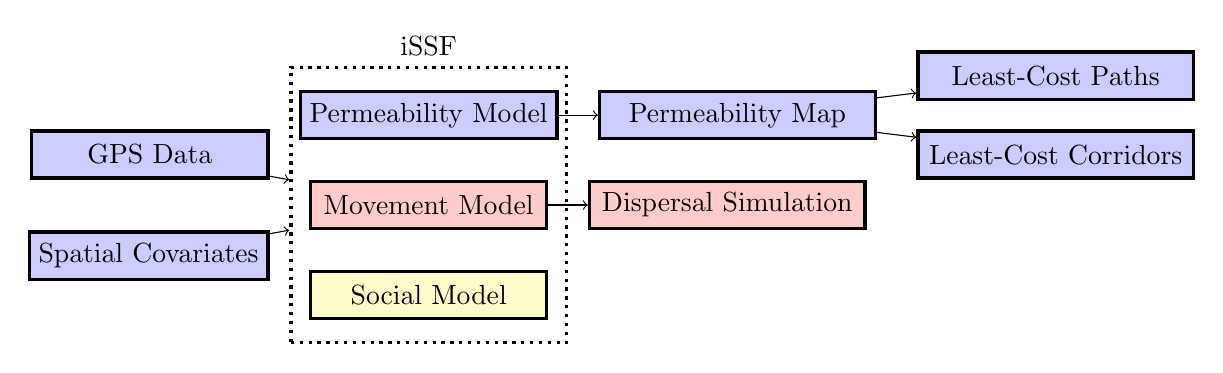
\begin{tikzpicture}[node distance=5mm and 5mm]
      \node (mod2) [nonterminal
        , minimum width = 30mm
        , fill          = red!20
        ] {Movement Model};
      \node (mod1) [nonterminal
        , above         = of mod2
        , fill          = blue!20
        , minimum width = 30mm
        ] {Permeability Model};
      \node (mod3) [nonterminal
        , below         = of mod2
        , fill          = yellow!20
        , minimum width = 30mm
        ] {Social Model};
      \node (dat1) [nonterminal
        , above left    = of mod2
        , fill          = blue!20
        , yshift        = -5mm
        , minimum width = 30mm
        ] {GPS Data};
      \node (dat2) [nonterminal
        , below left    = of mod2
        , fill          = blue!20
        , yshift        = +5mm
        , minimum width = 30mm
        ] {Spatial Covariates};
      \node (for1) [nonterminal
        , right         = of mod1
        , fill          = blue!20
        , minimum width = 35mm
        ] {Permeability Map};
      \node (forfor1) [nonterminal
        , right         = of for1
        , fill          = blue!20
        , minimum width = 35mm
        , yshift        = +5mm
        ] {Least-Cost Paths};
      \node (forfor2) [nonterminal
        , right         = of for1
        , fill          = blue!20
        , minimum width = 35mm
        , yshift        = -5mm
        ] {Least-Cost Corridors};
      \node (for2) [nonterminal
        , right         = of mod2
        , fill          = red!20
        , minimum width = 35mm
        ] {Dispersal Simulation};
      \node (box) [draw
        , dotted
        , very thick
        , minimum width   = 35mm
        , minimum height  = 35mm
        ] {};
      \node [above = of box, yshift = -5mm] {iSSF};
      \path (dat1) edge[->] (box);
      \path (dat2) edge[->] (box);
      \path (mod1) edge[->] (for1);
      \path (mod2) edge[->] (for2);
      \path (for1) edge[->] (forfor1);
      \path (for1) edge[->] (forfor2);
    \end{tikzpicture}
    \caption{Schematic overview of our methodological approaches. The blue boxes
    highlight our main line of work which resulted in the identification of
    least-cost paths and least-cost corridors. The red boxes show that we
    additionally used the iSSF framework to analyze movement behavior in more
    detail and to simulate dispersal events. Finally, the yellow box indicates
    our attempt to use the iSSF framework to model and analyze the influence of
    the social landscape on dispersal behavior.}
    \label{SchematicOverview}
  \end{center}
\end{figure}

\newpage
\subsection{Movement Model \& Dispersal Simulation}
\label{Appendix:DispersalSimulation}
\subsubsection{Methods}
To gain more detailed insights into the movement behavior of dispersing wild
dogs and to simulate dispersal events, we fitted a more complex movement model.
The movement model still contained the most parsimonious habitat selection
model, but in addition included interaction terms between movement metrics (i.e.
\(cos(ta)\), \(log(sl\))) and environmental covariates (e.g. water). For
instance, for the environmental covariate \textit{Water}, we created the
interaction terms \textit{cos(ta):Water} and \textit{log(sl):Water}. These
interactions served to learn how dispersers moved differently, depending on
environmental covariates (for comparable work see \cite{Prokopenko.2017}). We
applied the same modeling framework as explained in \Cref{Modeling} and ran
forward model selection based on AIC to identify the most parsimonious movement
model. That is, we departed from the habitat selection model and iteratively
added interactions with movement metrics. Note that we applied forward model
selection only on the newly identified interactions, but not for the terms that
were already in the habitat selection model. Since we attempted to keep our
simulation simple, we did not average models with positive AIC-weights but
simply identified the most parsimonious movement model.

Using the most parsimonious movement model, we simulated 1000 dispersal events
departing from the core study area. The simulation basically resembled an
inverted iSSF function and was set up as follows. First, we sampled a random
starting location within the core study area. Second, we assigned a random
orientation in order to be able to calculate turning angles. Third, we created
an array of 25 random steps (i.e. one stratum) following the same procedure as
described in \Cref{Modeling}. Fourth, we extracted environmental covariates
along each of the generated random steps and calculated the metrics listed in
\Cref{ExtractedCovars}. Fifth, we applied \Cref{EQ2} using parameter estimates
from the movement model and calculated the selection score \(w(x)\) of each of
the 25 random steps. Sixth, we identified and realized the step with the highest
selection score and determined the new location. We then repeated steps three to
six until 200 steps were realized. To deal with dispersers that approached a map
boundary, our simulation included the options to either stop the simulation and
skip to the next disperser, or to remove any random step ranging outside the
study area, thereby forcing the simulated disperser to stay within the
boundaries. None of the simulated dispersers approached a map boundary within
200 steps and the decision did not influence our findings. Although we ran the
simulation only for dispersers departing from the core study area, one could
easily expand the simulation to include multiple sources and thereby check how
well these sources are connected.

\newpage
\subsubsection{Results}
Along with the original covariates contained in the habitat selection model, our
most parsimonious movement model (see \Cref{ModelAICs2} and
\Cref{MovementModelResults}) retained three additional interactions (see red box
in \Cref{MovementModel}a). Since the sign and direction of the effects contained
in the habitat selection model did not markedly change, we only report on the
newly added interactions between environmental covariates and movement metrics.
For an easier interpretation of how these interactions influenced habitat
selection and movement patterns during dispersal, we prepared surface plots as
depicted in \Cref{MovementModel}b. These surface plots revealed that dispersers
preferred long steps (i.e. a high movement rate) when water cover was low,
whereas they preferred short steps (i.e. a low movement rate) when water cover
was high (see \Cref{MovementModel}b1). Furthermore, dispersers were indifferent
between high and low turning angles in proximity to water, but clearly preferred
low turning angles (i.e. a high \(cos(ta)\)) when distance to water was high
(see \Cref{MovementModel}b2). Finally, dispersers preferably realized steps with
low turning angles when human influence was low, whereas they preferably
realized low turning angles when human influence was high (see
\Cref{MovementModel}b3).

\begin{figure}[hbtp]
  \begin{center}
    \begin{tikzpicture}
        \node[anchor=south west,inner sep=0] (image) at (0,0,0) {
          \begin{minipage}{0.95\textwidth}
            \begin{center}
              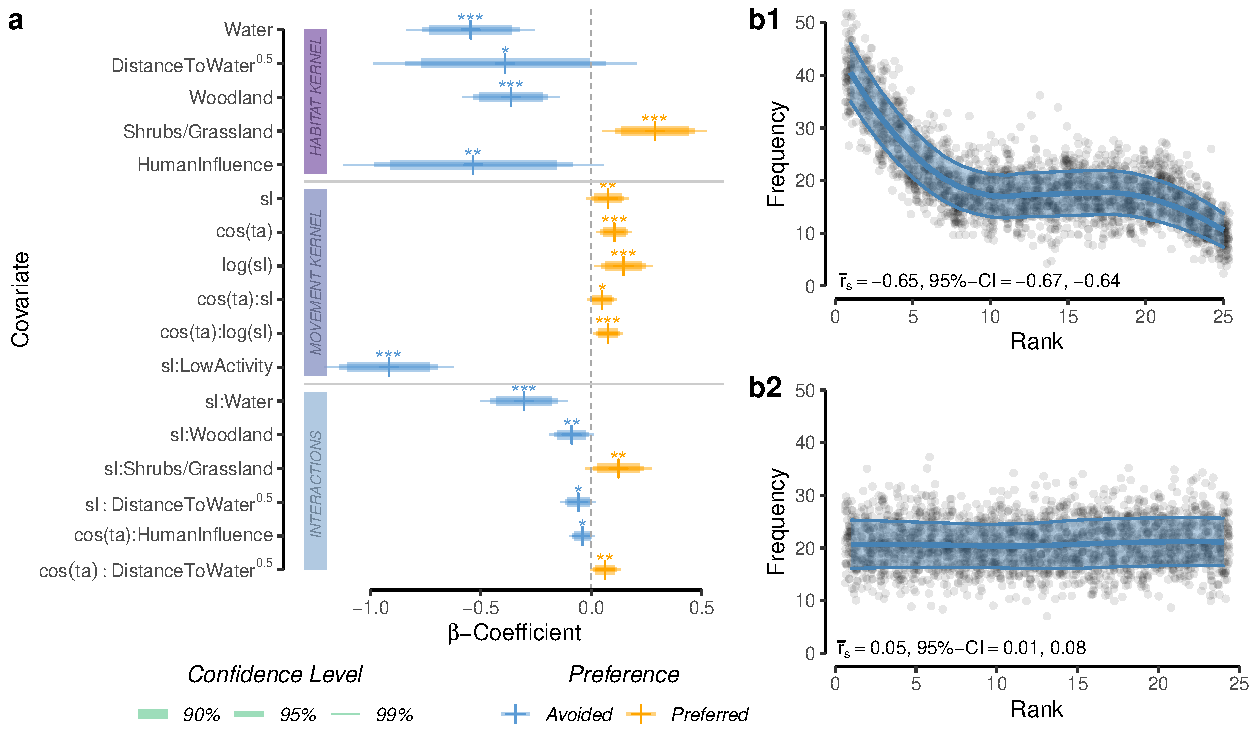
\includegraphics[width = 0.80\textwidth]
                {99_MovementModel.pdf}\\
              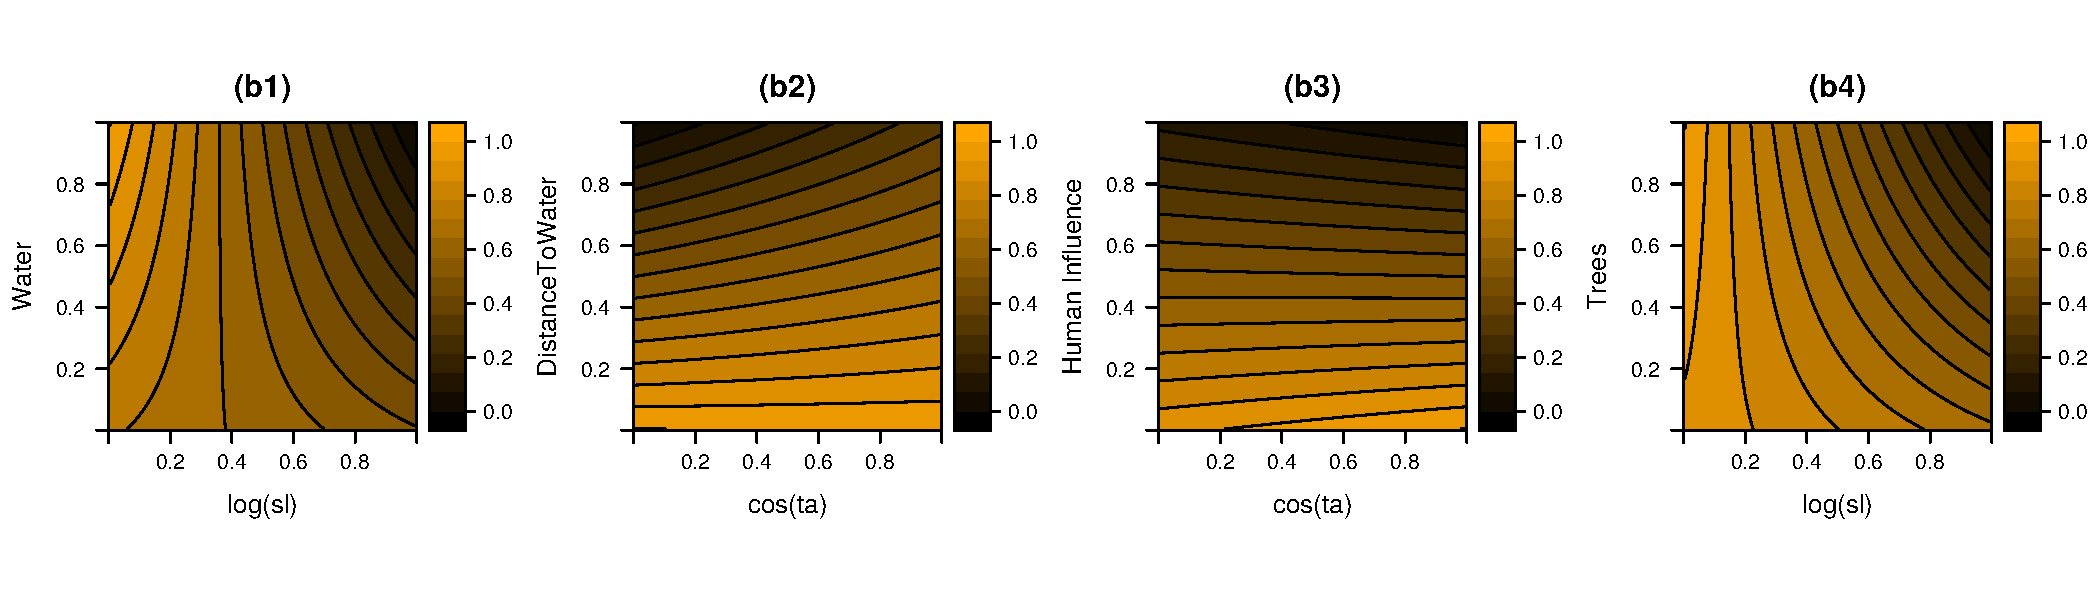
\includegraphics[width = 1\textwidth]
                {99_MovementModel(Interactions).pdf}
            \end{center}
          \end{minipage}
        };
        \begin{scope}[x={(image.south east)},y={(image.north west)}]
           %  % next four lines will help you to locate the point needed by
           %  % forming a grid. comment these four lines in the final picture.↓
           % \draw[help lines,xstep=.1,ystep=.1] (0,0) grid (1,1);
           % \draw[help lines,xstep=.05,ystep=.05] (0,0) grid (1,1);
           % \foreach \x in {0,1,...,9} { \node [anchor=north] at (\x/10,0) {0.\x}; }
           % \foreach \y in {0,1,...,9} { \node [anchor=east] at (0,\y/10) {0.\y};}
           %  % upto here
            \draw [red, dashed] (0.13, 0.50) rectangle (0.405, 0.645);
        \end{scope}
    \end{tikzpicture}
    \caption{(a) Results from the most parsimonious movement model. Negative
    coefficients indicate avoidance of a covariate, positive coefficients
    selection of a covariate. Whiskers delineate the 95\%-CIs for estimated
    parameters. The intercept is meaningless in the iSSF framework and was thus
    omitted. (b) Corresponding surface plots for two-way interactions. Light
    areas depict a combination of covariates that were preferred by dispersers,
    whereas darker areas correspond to avoided combinations. The absolute values
    along the axes have no meaning as original values were normalized to 0 (low)
    and 1 (high).}
    \label{MovementModel}
  \end{center}
\end{figure}

\newpage
\noindent \Cref{Simulations}a shows the outcome of the dispersal simulations.
For better visibility of high-frequency routes, we rasterized all simulated
trajectories and computed a heatmap depicting areas that were crossed by many
simulated trajectories. Unsurprisingly, we found that the dispersal trajectories
clearly reflected preferences that we identified earlier. For instance, most
trajectories were quite directional, avoided crossing a waterbody, ran along
water bodies and avoided human-dominated areas. More interestingly, however, the
resulting heatmap closely resembled our permeability surface (see
\Cref{Simulations}b). That is, areas providing high permeability were typically
crossed by more simulated trajectories. Yet, the heatmap also showed that some
regions are almost impossible to reach, even if they provide highly permeable
landscapes. For example, although the western section of the Okavango Delta
holds highly permeable landscapes, no simulated trajectory reached these areas.
In contrast, many trajectories ventured towards east, some of them even crossing
the border to Zimbabwe. The reason that no trajectory reached the eastern part
of the Delta is likely owed to severe human influence and an impermeable flood
that together posed an insurmountable barrier and prevented dispersers from
traversing the landscape.

\begin{figure}[h]
  \begin{center}
    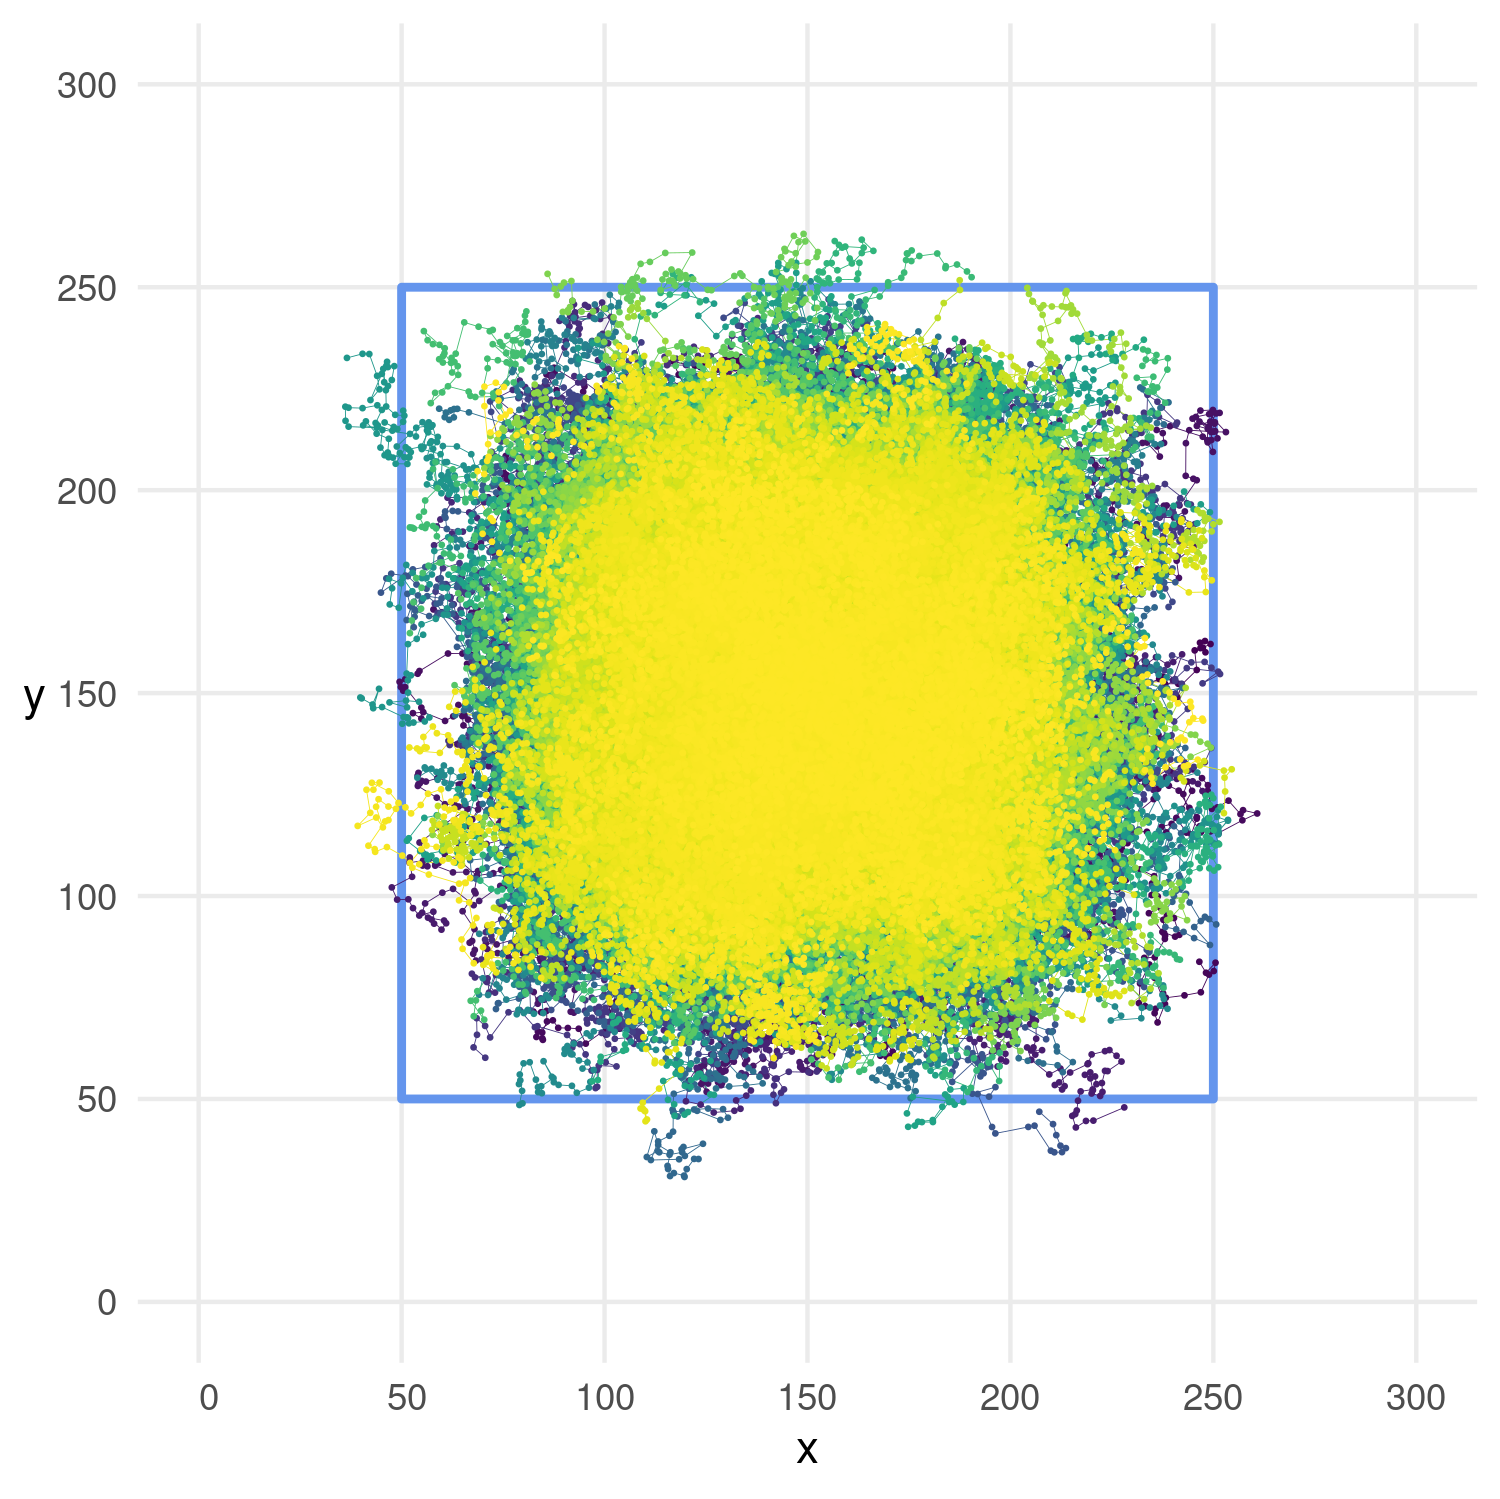
\includegraphics[width = 0.83\textwidth]{99_Simulations.pdf}
    \caption{(a) Heatmap of 1000 simulated dispersal events departing from the
    core study area (white rectangle) in northern Botswana (countries with
    dashed white lines). (b) Permeability map for the same extent to illustrate
    that simulated dispersal trajectories typically cover highly permeable
    landscapes.}
    \label{Simulations}
  \end{center}
\end{figure}

\newpage
\begin{table}[h]
  \caption{Results from the forward model selection procedure based on AIC
  \citep{Burnham.2002} for our movement model. Weights were calculated using:
  \(\text{AIC-Weight}_i = \frac{e^{-0.5} \Delta \text{AIC}_i} {\sum_{i = 1}^n
  e^{-0.5} \Delta \text{AIC}_i} \). (*) represents all covariates from the most
  parsimonious habitat selection model, i.e. \(cos(ta)\), \(log(sl\)),
  \textit{Water}, \textit{DistanceToWater}, \textit{Shrubs/Grassland},
  \textit{HumansBuff5000}, and \textit{Trees}. To keep the table short we only
  included models with positive AIC weights. We abstained from averaging models
  with AIC-weight \(>\) 0 because we attempted to keep our simulation simple.}
  \label{ModelAICs2}
  \begin{center}
    \resizebox{\textwidth}{!}{
      \begin{tabular}{llllll}
      \toprule
      \textbf{Covariates} &
        \textbf{AIC} &
          \textbf{\(\Delta\)AIC} &
            \textbf{AIC-Weight} &
              \textbf{LogLik} \\
      \midrule
      \rowcolor[gray]{0.80}
        (*),
        log(sl):Water, cos(ta):DistanceToWater, cos(ta):HumansBuff5000 &
          89814.19 &
            0.00 &
              0.13 &
                -44889.10 \\
        (*), log(sl):Water, cos(ta):DistanceToWater, cos(ta):Trees &
          89814.37 &
            0.17 & 0.12 &
              -44889.18 \\
        (*), log(sl):Water, cos(ta):DistanceToWater &
          89814.46 &
            0.27 &
              0.11 &
                -44890.23 \\
        (*), log(sl):Water, cos(ta):DistanceToWater, cos(ta):HumansBuff5000, cos(ta):Trees &
          89814.87 &
            0.68 &
              0.09 &
                -44888.44 \\
        (*), log(sl):Water, cos(ta):DistanceToWater, cos(ta):HumansBuff5000, cos(ta):Shrubs &
          89815.32 &
            1.13 &
              0.07 &
                -44888.66 \\
        (*), log(sl):Water, cos(ta):DistanceToWater, cos(ta):Shrubs &
          89815.34 &
            1.15 &
              0.07 &
                -44889.67 \\
        (*), log(sl):Water, cos(ta):DistanceToWater, cos(ta):HumansBuff5000, log(sl):Shrubs &
          89815.40 &
            1.20 &
              0.07 &
                -44888.70 \\
        (*), log(sl):Water, cos(ta):DistanceToWater, log(sl):Shrubs &
          89815.67 &
            1.48 &
              0.06 &
                -44889.84 \\
        (*), log(sl):Water, cos(ta):DistanceToWater, cos(ta):HumansBuff5000, log(sl):HumansBuff5000 &
          89815.94 &
            1.75 &
              0.05 &
                -44888.97 \\
        (*), log(sl):Water, cos(ta):DistanceToWater, cos(ta):HumansBuff5000, cos(ta):Trees, log(sl):Shrubs &
          89816.08 &
            1.89 &
              0.05 &
                -44888.04 \\
        (*), log(sl):Water, cos(ta):DistanceToWater, cos(ta):HumansBuff5000, log(sl):DistanceToWater &
          89816.14 &
            1.95 &
              0.05 &
                -44889.07 \\
        (*), log(sl):Water, cos(ta):DistanceToWater, cos(ta):HumansBuff5000, cos(ta):Water &
          89816.16 &
            1.97 &
              0.05 &
                -44889.08 \\
        (*), log(sl):Water, cos(ta):DistanceToWater, log(sl):HumansBuff5000 &
          89816.18 &
            1.99 &
              0.05 &
                -44890.09 \\
        (*), log(sl):Water, cos(ta):DistanceToWater, cos(ta):HumansBuff5000, log(sl):Trees &
          89816.19 &
            2.00 &
              0.05 &
                -44889.10 \\
      \bottomrule
      \end{tabular}
    }
  \end{center}
\end{table}

\begin{table}[h]
  \caption{Selection coefficients as derived from the most parsimonious movement
  model. The movement model was a modified habitat selection model to which we
  added additional interaction terms between movement metrics and environmental
  covariates (e.g. \(Water:cost(ta\_)\)) in order to learn about how movement
  behavior changes depending on the environmental covariates.}
  \label{MovementModelResults}
  \begin{center}
    \resizebox{0.5\textwidth}{!}{
      \begin{tabular}{llllll}
      \toprule
      Covariate & Coefficient & SE & p-value \\
      \midrule
      cos(ta) & 0.149 & 0.045 & 0.001 \\
      log(sl) & 0.053 & 0.019 & 0.005 \\
      Water & -0.265 & 0.090 & 0.003 \\
      DistanceToWater & -0.272 & 0.226 & 0.230 \\
      Shrubs & 0.391 & 0.082 & 0.000 \\
      HumansBuff5000 & -0.466 & 0.203 & 0.022 \\
      Trees & -0.177 & 0.072 & 0.013 \\
      log(sl):Water & -0.040 & 0.008 & 0.000 \\
      cos(ta):DistanceToWater & 0.115 & 0.038 & 0.003 \\
      cos(ta):HumansBuff5000 & -0.047 & 0.031 & 0.134 \\
       \bottomrule
      \end{tabular}
    }
  \end{center}
\end{table}

\newpage
\subsection{Social Model}
\label{Appendix:SocialLandscape}
\subsubsection{Methods}
We used GPS relocation data of resident wild dogs and calculated a
geo-referenced stack of layers to which we refer as the \textit{social
landscape}. The social landscape was a collection of raster-layers, each
depicting the probability of encountering a resident group in a given pixel and
month. The social landscape was updated every month, using a moving window that
took into account six months of relocation data. For instance, the social
landscape dated July 1\textsuperscript{st} consisted of GPS relocation data
collected between January 1\textsuperscript{st} and June 30\textsuperscript{th}.
Because we collected relocation data of residents only inside the core study
area, we modeled the social landscape only for this region. GPS relocations were
collected at a 24-hourly interval during residence, so we kept one GPS
relocation per pack and day. To compute monthly updated social landscapes, we
calculated each resident pack's utilization distribution (UD) and corresponding
95\% home range (HR) using the kernelUD function from the R-package
\textit{adehabitatHR} \citep{Calenge.2019}. The package required to set a
smoothing parameter \(h\), which determined the sharpness of the resulting UD
and 95\%-HR. To come up with a meaningful smoothing parameter \(h\), we followed
the procedure described in \cite{Cozzi.2018}. That is, we first applied the
reference value \( h_{ref} \), which the package automatically determined. We
then obtained the corresponding UD and 95\%-HR and assessed whether the 95\%-HR
comprised of a single polygon or whether it split up into multiple polygons. In
case the 95\%-HR segregated into multiple polygons, we assumed that the
smoothing parameter was set to strictly. On the other hand, if the 95\%-HR
comprised of a single polygon, we assumed that we could further tighten the
smoothing parameter. We thus iteratively adjusted the smoothing parameter until
a value right before the 95\%-HR split up into multiple polygons. However, we
maximally varied \( h \) within 30\% and 120\% of the original \( h_{ref} \) to
avoid extreme over- or under-smoothing. Using the resulting \(h\) we computed
the final UD and corresponding 95\%-HR. Each pack's UD of a given month was
converted to a spatial probability density using \(f(x) =
\frac{x_i}{\sum_1^n{x_i}}\), so that pixel-values summed up to one. We then used
\Cref{EQ4} to merge all UDs of the same month and to calculate the probability
of not encountering any wild dogs in a given pixel and month.

\begin{equation}
\label{EQ4}
x_i = 1 - \prod_{j = 1}^{n} (1 - x_{ij})
\end{equation}

\noindent where \(x_i =\) is the probability of encountering another pack in
pixel \(i\) and \(x_{ij} =\) the probability of encountering pack \(j\) in pixel
\(i\). Finally, we inverted this probability using \((1-x_i)\) to get the
probability of encountering at least one resident pack in a given pixel and
month. Note that we kept track of each packs' 95\%-HR throughout all months,
which allowed us to identify through which HRs dispersers moved during
dispersal. An example of the final layers is given in
\Cref{SocialLandscapeExample}.

\begin{figure}[h]
  \begin{center}
    \includegraphics[width = 0.95\textwidth]{99_SocialLandscapeExample.pdf}
    \caption{(a) Example of a layer depicting the probability of encountering a
    resident pack in July 2017. The layer was derived from utility distributions
    of all packs residing in the core study area. (b) Example of a layer
    depicting all 95\% home ranges of the packs residing in the core study area.
    This layer served to identify whether a disperser still moved through his
    natal pack's home range, or whether it moved through a foreign packs home
    range. The layers in (a) and (b) were updated each month to take into
    account only the latest GPS relocation data of resident individuals.}
    \label{SocialLandscapeExample}
  \end{center}
\end{figure}

\noindent To fit a social model using the newly created social landscape, we
reran our iSSF described in \Cref{Modeling}. However, this time we discarded any
stratum that did not fully lie within the core study area. The social model that
we fitted was again a modification of the most parsimonious habitat selection
model. Despite the covariates contained in the habitat selection model, we added
the social covariates listed in \Cref{SocialCovars}. Because we hypothesized
that the preference for encountering other wild dogs was different within and
outside the disperser's natal home range, we included the interaction terms
\textit{ProbEncounter:OwnHomerange} and \textit{ProbEncounter:ForeignHomeranges}
in the social model. Since we did not anticipate to use the model for
predictions, we did not engage in model selection.

\begin{table}[h]
  \begin{center}
    \caption{Overview of extracted social covariates. Values were extracted from
    the layer that was closest in date to the actual step.}
    \label{SocialCovars}
    \resizebox{\textwidth}{!} {
      \begin{tabular}{lllll}
      \hline
      \textbf{Category} &
        \textbf{Covariate} &
          \textbf{Description} &
            \textbf{Values} \\
              % \textbf{Source(s)} \\
      \midrule
      Social Features
        & OwnHomerange
          & Percentage cover of natal pack’s 95\% home-range along step
            & 0-100\% \\
      Social Features
        & ForeignHomeranges
          & Number of foreign packs’ 95\% home-ranges along step
            & \(\geq\) 0 \\
      Social Features
        & ProbEncounter
          & Average probability of encountering conspecifics along step
            & 0-100\% \\
      \hline
      \end{tabular}
    }
  \end{center}
\end{table}

\newpage
\subsubsection{Results}
Results from our social model are depicted in \Cref{SocialModel}a (see also
\Cref{SocialModelResults}). Again, parameter estimates for the covariates
contained in the habitat selection model did not severely change and we will
only report on the newly added social covariates (see red box in
\Cref{SocialModel}a). Visual inspection of the corresponding surface plot (see
\Cref{SocialModel}b1) revealed that dispersers tried to maximize the probability
of encounter when moving outside their natal pack's HR. Yet, this preference was
even stronger when dispersers moved inside their natal pack's HR. A second
surface plot (see \Cref{SocialModel}b2) showed that dispersers maximized the
probability of encounter when the number of foreign HRs was low, but that they
minimized the probability of encounter when the number of foreign HRs was high.
In summary, dispersers appeared to be drawn towards other wild dogs, but only if
the number of overlapping foreign HRs was low.

\begin{figure}[hbtp]
  \begin{center}
    \begin{tikzpicture}
        \node[anchor=south west,inner sep=0] (image) at (0,0,0) {
          \begin{minipage}{0.95\textwidth}
            \begin{center}
              \includegraphics[width = 0.75\textwidth]
                {99_SocialModel.pdf}\\
              \includegraphics[width = 0.8\textwidth]
                {99_SocialModel(Interactions).pdf}
            \end{center}
          \end{minipage}
        };
        \begin{scope}[x={(image.south east)},y={(image.north west)}]
           %  % next four lines will help you to locate the point needed by
           %  % forming a grid. comment these four lines in the final picture.↓
           % \draw[help lines,xstep=.1,ystep=.1] (0,0) grid (1,1);
           % \draw[help lines,xstep=.05,ystep=.05] (0,0) grid (1,1);
           % \foreach \x in {0,1,...,9} { \node [anchor=north] at (\x/10,0) {0.\x}; }
           % \foreach \y in {0,1,...,9} { \node [anchor=east] at (0,\y/10) {0.\y};}
           %  % upto here
            \draw [red, dashed] (0.15, 0.60) rectangle (0.43, 0.75);
        \end{scope}
    \end{tikzpicture}
    \caption{(a) Estimated parameters from the social model. Negative
    coefficients indicate avoidance of a covariate, positive coefficients
    selection of a covariate. Whiskers delineate the 95\%-CIs for estimated
    parameters. The intercept is meaningless in the iSSF framework and was thus
    omitted. (b) Corresponding surface plots for two-way interactions (red box).
    Light areas in the surface plots depict preferred combinations of the
    covariates, whereas darker areas correspond to avoided combinations. The
    absolute values along the axes have no meaning as original values were
    normalized to 0 (low) and 1 (high).}
    \label{SocialModel}
  \end{center}
\end{figure}

\newpage
\begin{table}[h]
  \caption{Selection coefficients as derived from the social model. The social
  model was a modified habitat selection model to which we added additional
  social covariates in order to learn about how the social landscape infleunces
  dispersal behavior.}
  \label{SocialModelResults}
  \begin{center}
    \resizebox{0.6\textwidth}{!}{
      \begin{tabular}{llllll}
        \toprule
        Covariate & Coefficient & SE & p-value \\
        \midrule
        cos(ta) & 0.148 & 0.066 & 0.025 \\
        log(sl) & 0.055 & 0.019 & 0.003 \\
        Water & -0.472 & 0.113 & 0.000 \\
        DistanceToWater & -0.193 & 0.411 & 0.639 \\
        Shrubs & 0.470 & 0.110 & 0.000 \\
        HumansBuff5000 & -1.013 & 0.295 & 0.001 \\
        Trees & -0.465 & 0.193 & 0.016 \\
        ProbEncounter & 0.724 & 0.268 & 0.007 \\
        OwnHomerange & 0.056 & 0.095 & 0.557 \\
        ForeignHomeranges & -0.099 & 0.132 & 0.452 \\
        ProbEncounter:OwnHomerange & 0.189 & 0.179 & 0.291 \\
        ProbEncounter:ForeignHomeranges & -0.504 & 0.281 & 0.072 \\
        \bottomrule
      \end{tabular}
    }
  \end{center}
\end{table}

\newpage
\subsection{Statutory Declaration}
I assure that this thesis is a result of my personal work and that no other than
the indicated aids have been used for its completion. Furthermore, I assure that
all quotations and statements that have been inferred literally or in a general
manner from published or unpublished writings are marked as such. Beyond this, I
assure that the work has not been used, neither completely nor in parts, to pass
any previous examination.\\
\vspace{15mm}\\
Zürich, \today

\vspace{5mm}

\includegraphics[width = 0.2\textwidth]{Signature.png}

\noindent David Hofmann

\end{document}
